% CLASE
\documentclass[a4paper,12pt]{article}

% PREÁMBULO
% Paquetes:
\usepackage[spanish]{babel}
\usepackage{csquotes}
\usepackage{graphicx}
\usepackage{tikz,color}
\usepackage{pgf-pie}
\usepackage{pgfgantt}
\usepackage{pdflscape}
\usepackage[backend=biber]{biblatex}
\usepackage[table]{xcolor}
\usepackage{multirow}
\usepackage{adjustbox}
\usepackage{wrapfig}
% Permite cortar las URL largas en cualquier caracter (se carga despues de
% biblatex, que ya trae el paquete url, para poder redefinir sus cortes).
\usepackage{xurl}

% Habilita los cortes de URL dentro de la bibliografia generada por biblatex.
\setcounter{biburlnumpenalty}{9000}
\setcounter{biburlucpenalty}{9000}
\setcounter{biburllcpenalty}{9000}
% Afloja el ajuste de linea unicamente dentro de la bibliografia, donde las URL
% largas dejan renglones sin puntos de corte utiles.
\appto{\bibsetup}{\emergencystretch=1em}

% Separacion vertical equivalente a una linea en blanco.
% Sustituye el uso de \newline o \\ al cierre de un parrafo, que dejaba una
% linea vacia y provocaba avisos "Underfull \hbox (badness 10000)".
\newcommand{\saltolinea}{\par\vspace{\baselineskip}}
\bibliography{Recursos/Bibliografia}

% CUERPO
\begin{document}

% Caratula
    \begin{titlepage}
        \centering
        
\includegraphics[width=0.2\textwidth]{Imagenes/LogoUTN.png}\par
        \vfill
        {\bfseries\LARGE Universidad Tecnológica Nacional \par}
        \vfill
        {\scshape\Large Facultad Regional Rosario \par}
        \vfill
        {\scshape\Huge Aplicación de Apoyo al Cuidado de Personas \par}
        \vfill
        {\itshape\Large Ingeniería en Sistemas de Información \par}
        {\itshape\Large Proyecto Final de Carrera \par}
        \vfill
        {\Large Autores: \par}
        {\Large Carignani, Esteban Agustín \par}
        {\Large Culich, María Agustina \par}
        {\Large Montisori, Agustín \par}
        \vfill
        {\Large Tutor: \par}
        {\Large Stortoni, Silvia \par}
        \vfill
        {\Large Agosto 2026 \par}
    \end{titlepage}

% Abstract
    \begin{abstract}
        Cuidar de otra persona, ya sea un adulto mayor, 
        un niño, una persona con discapacidad o alguien 
        con una enfermedad, puede ser una tarea compleja. 
        La gestión de medicamentos, horarios, cuidadores, 
        turnos, recordatorios médicos y la comunicación
        entre las personas involucradas son parte de
        la carga diaria que ello implica.
        Basándonos en las respuestas de una encuesta realizada enfocada a personas que tienen a su cargo el cuidado de otras, presentamos una aplicación móvil innovadora que facilita la gestión y organización de las tareas que implica estar al cuidado de alguien más. Nuestra propuesta es una app que permitiría el registro de información personal de la persona bajo cuidado y la asociación de esta al cuidador, centralización de la comunicación entre ambas partes y terceros involucrados, simplicidad en la organización de visitas y turnos médicos, agenda de medicación, tareas cotidianas, etc. Además, se incluirán herramientas que respondan a las necesidades relevadas en el cuestionario de sondeo.
    \end{abstract}

    \newpage

% Tabla de contenidos
    \tableofcontents 
    
    \newpage

% Análisis de la organización
    \section{Análisis de la organización}
    \par Partiendo de la base en que para el proyecto no existe una organización u empresa definida particular en la cuál apoyarnos, el análisis organizacional que llevaremos a cabo pone foco principal en el equipo de desarrollo del proyecto en cuestión, considerando al mismo como una \textit{startup} que se inicia en el mercado de desarrollo de soluciones informáticas. Concentrando los esfuerzos principalmente en las capacidades y recursos del equipo a cargo.
    \par El objetivo es evaluar la estructura del equipo, habilidades, procesos de trabajo, disponibilidad de recursos financieros y tecnológicos, definición de fortalezas, debilidades y oportunidades que pueden afectar al desarrollo del equipo como organización.
    \subsection{Bubisoft}
    \par La empresa toma como punto de partida inicial el desarrollo de soluciones informáticas orientadas a problemáticas sociales y cotidianas de las personas.
    \par El mercado al que apunta la organización y sobre el cual sienta las bases de su crecimiento es el siguiente:
    \begin{itemize}
        \item Sujetos que se enfrentan ante una situación específica que deriva en la necesidad de tener una o más personas encargadas.
        \item Familiares o red de contención que se encargan del cuidado de una o más personas dependientes o parcialmente dependientes y de todas las tareas que engloba.
    \end{itemize}
    \par Tomando esto en consideración, procedemos a la realización del análisis que nos permite determinar la misión, visión y objetivos de la organización.
    \subsection{Misión}
    \par Brindar soluciones tecnológicas que simplifiquen la atención a las problemáticas cotidianas para aquellas personas que se encuentren en situación de vulnerabilidad y sirvan de apoyo para con los responsables del cuidado.
    \subsection{Visión}
    \par Posicionarse como una de las principales consultoras tecnológicas responsables de brindar soluciones informáticas innovadoras para abordar diversas problemáticas sociales.
    \subsection{Objetivos principales}
    \begin{itemize}
        \item Brindar soluciones tecnológicas que mejoren la calidad de vida de las personas mayores y faciliten la labor de sus cuidadores.
        \item Alcanzar la sostenibilidad financiera y un crecimiento rentable a largo plazo, posicionándose de forma estratégica en el mercado de soluciones informáticas.
        \item Contribuir a mejorar el bienestar general de la sociedad, estudiando y evaluando con atención sus necesidades y contribuyendo con formas de satisfacerlas a través del desarrollo de nuevas tecnologías.
    \end{itemize}
    \subsection{Objetivos secundarios}
    \begin{enumerate}
        \item \underline{Organizacionales}
        \begin{itemize}
            \item Identificar las necesidades específicas de las personas.
            \item Desarrollar soluciones tecnológicas fáciles de usar e intuitivas para los usuarios.
            \item Ofrecer funcionalidades que aborden las necesidades más comunes.
            \item Desarrollar un sólido modelo de negocio que genere ingresos a través de suscripciones.
            \item Atraer y retener usuarios.
            \item Explorar oportunidades de expansión en mercados similares.
        \end{itemize}
        \item \underline{Sociales}
        \begin{itemize}
            \item Reducir la carga de trabajo de los cuidadores y familiares.
            \item Promover la independencia y autonomía de las personas mayores.
            \item Reducir los niveles de aislamiento social y soledad de las personas mayores.
            \item Concientizar a la sociedad sobre los desafíos que representan la etapa de envejecimiento.            
        \end{itemize}
    \end{enumerate}
    \subsection{Organigrama}
    \par Si bien la empresa resulta ser una startup inicial que consta de pocas personas integrándola, realizamos el organigrama basándonos en los roles y funciones que cumplen sus integrantes.
    \par\noindent 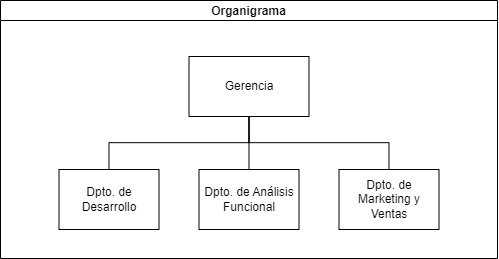
\includegraphics[width=1\textwidth]{Imagenes/Organigrama.jpg}
    \par Profundizaremos un poco más en las tareas a cargo de cada uno de los departamentos que integran a la empresa.
    \begin{itemize}
        \item[\textbf{Gerencia:}] Se compone del equipo fundador de la empresa, encargados de la toma de decisiones relacionadas al futuro de la empresa, el camino a seguir y los proyectos a encarar.
        \item[\textbf{Desarrollo:}] Es el departamento a cargo del arquitecto de software, quien coordina a todos los desarrolladores a lo largo de la codificación, desarrollo y mantenimiento del software.
        \item[\textbf{Análisis:}] Este departamento está a cargo del líder de proyectos, a su mando están los analistas y testers, encargados de relevar, comprender e interpretar las necesidades de los clientes y asegurar que las mismas se satisfagan correctamente por el software implementado.
        \item[\textbf{Marketing:}] El departamento de marketing se encarga de publicitar, publicar y promover el uso de la aplicación desarrollada. A su vez, sus tareas incluyen realizar campañas de retención de usuarios, escuchando las críticas que estos ofrezcan, y comunicándolas al departamento de análisis. 
    \end{itemize}
    \subsection{Matriz FODA}
    \textbf{\underline{Fortalezas}}
    \begin{itemize}
        \item[] \textit{Enfoque en problemática social:} Al centrarse en atender una necesidad real y creciente de la sociedad, la empresa da un propósito claro, apuntado a un mercado real de potenciales clientes.
        \item[] \textit{Soluciones innovadoras:} La empresa propone soluciones tecnológicas novedosas y adaptadas a las necesidades específicas de las personas.
        \item[] \textit{Potencial de impacto:} Las soluciones tienen el potencial de mejorar significativamente la calidad de vida de las personas, generando un impacto positivo en la sociedad.
        \item[] \textit{Alta motivación:} Al ser una empresa que está en sus inicios, sus integrantes están altamente motivados para enfrentar los diferentes desafíos de forma proactiva e inmediata.
    \end{itemize}
    \textbf{\underline{Oportunidades}}
    \begin{itemize}
        \item[] \textit{Innovación:} Los nuevos avances en tecnología como la inteligencia artificial y la domótica pueden abrir nuevas posibilidades para el desarrollo de soluciones innovadoras.
        \item[] \textit{Creciente mercado:} De la mano con la revolución tecnológica y el amplio rango de edad que abarcan actualmente las tecnologías, genera una demanda cada vez mayor de soluciones que puedan hacer frente a las necesidades de las personas.
        \item[] \textit{Alianzas estratégicas:} La organización es capaz de asociarse con otras empresas, organizaciones o instituciones enfocadas en temáticas inherentes a las soluciones brindadas, para ampliar su alcance y potenciar su impacto.
    \end{itemize}
    \textbf{\underline{Debilidades}}
    \begin{itemize}
        \item[] \textit{Inexperiencia:} Al ser una startup reciente que incursiona en el desarrollo de soluciones tecnológicas, se enfrenta a los problemas de falta de experiencia a la hora de afrontar desafíos técnicos, financieros y de gestión.
        \item[] \textit{Capital limitado:} Cada decisión a tomar implica un potencial riesgo en la continuidad y estabilidad de la empresa debido al poco capital inicial con el que cuentan.
        \item[] \textit{Escasez de recursos:} El escaso nivel de personal inicial representa una limitante a la hora de tomar posibles proyectos debido al riesgo de caer en una sobrecarga laboral que afecte a las entregas y el éxito de los mismos.
    \end{itemize}
    \newpage
    \textbf{\underline{Amenazas}}
    \begin{itemize}
        \item[] \textit{Avances tecnológicos:} La aparición de nuevas tecnologías pueden crear soluciones a las mismas problemáticas de los proyectos realizados por la empresa pudiendo dejarlos obsoletos.
        \item[] \textit{Dificultades para obtener financiación:} sin el apoyo de programas gubernamentales y organizaciones sin fines de lucro, podría limitar la capacidad de la organización para crear nuevas soluciones.
        \item[] \textit{Mercado competitivo:} El gran nivel de demanda y competencia salarial que presenta el actual mercado de tecnología, dificulta el ingreso competitivo y la rentabilidad inmediata de la empresa.
    \end{itemize}
    \subsection{Procesos principales}
    Tomando en consideración el análisis hecho de la organización, y el foco que hacen en las problemáticas sociales, consideramos los siguientes procesos principales.

    \noindent \textbf{\underline{Investigación y desarrollo}}

    Dentro de los procesos de investigación y desarrollo incluimos procesos más atómicos como:
    \begin{itemize}
        \item[] \textit{Identificación de necesidades:} este proceso engloba la realización de un análisis de las necesidades específicas de los stakeholders tanto a nivel individual como a nivel colectivo. Dentro del mismo se engloban tareas como la realización de encuestas, entrevistas, grupos focales, etc., que permitan comprender los desafíos y oportunidades que enfrentan.
        \item[] \textit{Diseño y modelado de soluciones:} consiste en diseñar las posibles soluciones tecnológicas innovadoras que hagan frente a las necesidades identificadas previamente, priorizando la facilidad de uso y las capacidades de los usuarios a los que apunta. Se emplean metodologías de modelado centradas en la experiencia de usuario para asegurar la conformidad y usabilidad de las aplicaciones.
        \item[] \textit{Desarrollo de software:} este proceso engloba todas las tareas relacionadas a la materialización de las propuestas tecnológicas planteadas y diseñadas previamente. Se definen y emplean metodologías de desarrollo acordes a las necesidades de cada proyecto y herramientas modernas, asegurando la calidad, seguridad y confiabilidad de las soluciones. Además se incluyen las tareas relacionadas al testing y pruebas para garantizar que las soluciones funcionen correctamente y cumplan con los requisitos establecidos.
    \end{itemize}

    \noindent \textbf{\underline{Implementación y soporte}}

    Este proceso engloba la salida y puesta en producción de las aplicaciones desarrolladas, junto con el seguimiento y mejora continua de las mismas, atendiendo a las necesidades de los usuarios y las opiniones recibidas.
    \begin{itemize}
        \item[] \textit{Implementación:} engloba el lanzamiento y puesta en producción de las soluciones tecnológicas en los entornos donde se utilizarán, brindando capacitación y asistencia a los usuarios para garantizar una adopción exitosa. Además se pautan mecanismos de seguimiento y evaluación para medir el impacto de las soluciones y realizar mejoras continuas.
        \item[] \textit{Soporte técnico:} consiste en brindar soporte técnico a los usuarios, resolviendo problemas de manera oportuna y eficiente. Para su efectividad, se utilizan canales de comunicación efectivos previamente definidos como información de contacto, opiniones y valoración en plataformas de descargas, etc.
        \item[] \textit{Actualizaciones y mantenimiento:} abarca las tareas enfocadas en actualizaciones periódicas de las soluciones tecnológicas para incorporar nuevas funcionalidades, corregir errores y mejorar el rendimiento.
    \end{itemize}

    \noindent \textbf{\underline{Gestión y administración}}

    Los procesos de gestión y administración son aquellos que alinean los objetivos estratégicos de la empresa con la visión y misión de las mismas, a fin de orientar los esfuerzos colectivos hacia una misma meta.
    \begin{itemize}
        \item[] \textit{Planificación estratégica:} consiste en establecer un plan estratégico que defina los objetivos a largo plazo de la startup, las estrategias para alcanzarlos y los recursos necesarios. Se realizan revisiones periódicas del plan para adaptarlo a las condiciones cambiantes del mercado y las necesidades de los usuarios.
        \item[] \textit{Gestión financiera:} engloba la gestión de los recursos financieros de manera eficiente, asegurando la sostenibilidad de la startup a largo plazo. Realizando periódicamente presupuestos, control de gastos y análisis de rentabilidad que sirvan de apoyo a la hora de tomar decisiones financieras.
        \item[] \textit{Gestión del talento humano:} abarca las tareas relacionadas al reclutamiento, evaluación, selección y capacitación de personal que formará parte de la empresa.
    \end{itemize}

    \noindent \textbf{\underline{Marketing y ventas}}

    Este proceso engloba todas aquellas tareas relacionadas a la divulgación, promoción y alcance de las soluciones tecnológicas puestas en el mercado. A su vez, engloba la definición de estrategias y planes para potenciar el alcance de la marca y su posicionamiento estratégico en el mercado.
    \begin{itemize}
        \item[] \textit{Estrategia de marketing:} se establece una estrategia publicitaria que permita dar a conocer las soluciones tecnológicas a los usuarios potenciales y generar interés en su adopción. Los principales canales de difusión consisten en la publicidad digital y la valoración en plataformas de descargas.
        \item[] \textit{Ventas:} consiste en la definición de un proceso de ventas efectivo que permita convertir a los clientes potenciales en usuarios reales. Incluye demostraciones de casos de éxito, pruebas gratuitas y planes de suscripción.
        \item[] \textit{Atención al cliente:} abarca los servicios de atención al cliente para fidelizar a los usuarios y resolver sus inquietudes.
    \end{itemize}

    \noindent \textbf{\underline{Evaluación y mejora continua}}

    Este proceso consiste en monitorear el impacto de las soluciones tecnológicas en la calidad de vida de las personas alcanzadas, utilizando indicadores clave de rendimiento (KPIs) para medir el éxito de las soluciones e identificar áreas de mejora.
    Además, se implementa un proceso de mejora continua capaz de optimizar las soluciones tecnológicas, los procesos internos y las estrategias de negocio, haciendo uso y beneficio de la retroalimentación de los usuarios y los datos recopilados.

    \newpage

% Analisis de problemas
    \section{Análisis de problemas}
    \par El surgimiento de la iniciativa de realizar un software que se encargue de la gestión y organización de las tareas que implica estar al cuidado de otras personas, se origina en las complejas problemáticas con las que nos encontramos diariamente.
    \par A fin de poder abordarlas con mayor exactitud y precisión, llevamos a cabo la realización de un cuestionario presentado a unas cincuenta personas, de diferentes edades, oficios y calidades de vida, con preguntas orientadas a sus experiencias en el cuidado de adultos mayores, niños pequeños, personas con alguna condición específica, etc. A partir del mismo, analizamos los resultados y concluimos en las diferentes problemáticas comunes.
    \saltolinea
    \subsection{Gráficas de respuestas}
    \par En esta sección presentamos las diferentes gráficas correspondientes a cada una de las preguntas realizadas en el relevamiento, que permiten posteriormente identificar potenciales usuarios, problemáticas, funcionalidades, etc.
    \par El relevamiento fue orientado a aquellas personas que se encuentran en posición de cuidador, ya sea profesionalmente o por algún vínculo en especial.
    \subsubsection{¿Qué vínculo o relación tienen?}
    \par El objetivo de la pregunta era comprender el tipo de vínculo que se mantuvo con la persona al cuidado para comprender de una mejor forma las siguientes respuestas y ver a qué público se puede orientar la solución que proponemos.
    \par Obtuvimos cincuenta y siete respuestas muy variadas, para realizar el análisis de los datos traspasamos la información para que sea más estructurada y homogénea, de esta forma se eliminaron inconsistencias, se corrigieron errores ortográficos y se igualaron los formatos de escritura.
    \par Los datos obtenidos quedaron distribuidos como se ve en el siguiente gráfico de torta. \newline
        \begin{tikzpicture}
            \pie[explode={0.2, 0.2, 0.2, 0.2, 0.2, 0.2, 0.2}]
            {35/Familiar, 
            26/Hijos, 
            14/Cuidador, 
            7/Docente, 
            7/Padres, 
            7/Niñeros, 
            4/Hermanos}
        \end{tikzpicture} 
    \saltolinea
    \par En la categorización de los tipos de vínculos se estableció que cuando se habla de “Padres”, se hace referencia a que la persona que contestó la encuesta tiene a cargo a sus hijos, en cambio cuando se dice “Hijos”, los participantes del cuestionario referían a que cuidaron a sus padres.
    \par Teniendo en cuenta los datos del cuestionario, se desprende el siguiente análisis:
    \begin{itemize}
        \item El 65\% de las personas que contestaron la encuesta se encuentran o encontraban al cuidado de algún familiar, dentro de esta categorización se encuentran familiares, hijos y hermanos. Esto nos revela que la mayoría de las personas que realizan las tareas de administración y cuidado no son profesionales.
        \item El 7\% contestaron que son padres y tienen al cuidado a sus hijos, diferenciamos esta categoría de la de los familiares porque se entiende teniendo en cuenta todas las respuestas del cuestionario que son menores de edad, mientras que en la categoría de familiares se hace referencia a mayores de edad.
        \item El 28\% contestaron que son personas externas a la familia de la persona que se encarga del cuidado. Entre ellos se encuentran cuidadores, niñeros y docentes.
    \end{itemize}
    \subsubsection{¿Cuáles son las principales problemáticas que enfrentan?}
    \par El objetivo de la pregunta era conocer cuáles eran las principales problemáticas, inconvenientes y dificultades con las que se encuentran los cuidadores.
    \par En este caso las personas que respondieron, realizaron distintos abordajes a la pregunta y al igual que en la pregunta anterior se realizó una limpieza y normalización de los datos de las respuestas. En este caso se registraron cincuenta y tres respuestas.
    \newline
        \begin{adjustbox}{max width=\textwidth}
        \begin{tikzpicture}
            \pie[explode={0.2, 0.2, 0.2, 0.2, 0.2, 0.2, 0.2, 0.2, 0.2}]
            {30/Cansancio y disponibilidad, 
            14/Comunicación, 
            14/Desconocimiento, 
            12/Organización, 
            12/Responsabilidad, 
            7/No responde, 
            5/Daños y enfermedades, 
            4/Movilidad y entorno, 
            2/Cuidadores}
        \end{tikzpicture}
        \end{adjustbox} 
    \saltolinea
    \par En primer lugar, teniendo en cuenta las respuestas, el análisis que podemos hacer sobre las principales problemáticas que están relacionadas con el cansancio, disponibilidad de tiempos, desconocimiento, organización, enfermedades; se vinculan directamente con la \textit{“pregunta 2: ¿Qué vínculo/relación tienen o tenían?”} donde la mayoría son familiares de las personas que están al cuidado, por lo que tiene sentido que su principal tarea no sea la de brindar cuidado o asistencia a sus allegados, si no que lo realicen en conjunto con las actividades diarias que tiene cada uno.
    \par Las otras temáticas como la responsabilidad, dañarse y movilidad se relacionan con las personas que contestaron y pertenecen al grupo de cuidadores externos a la familia. Tienen que ver con las problemáticas y preocupaciones que intervienen en sus trabajos.
    \par Por otro lado, se registraron dos problemáticas relacionadas con la comunicación:
    \begin{itemize}
        \item La primera y más frecuente en las respuestas, se relaciona con la comunicación que se da entre las personas que se encargan de cuidar. Esta dificultad en la comunicación hace que se pierda información, se malinterprete y provoque dobles esfuerzos o problemáticas posteriores para la persona al cuidado.
        \item La segunda describe la comunicación entre el cuidador y la persona al cuidado. Esto ocurre generalmente cuando la persona al cuidado no puede expresar concretamente cuáles son sus necesidades y el diálogo es complejo.
    \end{itemize}
    \par Las problemáticas de entorno y cuidadores representan únicamente dos respuestas que hacen referencia a inconvenientes relacionados con terceros, en cuanto al entorno, la persona que registró la respuesta detalló que se ven involucrados muchos problemas con obras sociales, trámites, tratamientos e incluso con familiares de la persona. Cuando se habla de cuidadores en otra respuesta, la persona expresó que tuvo varios inconvenientes con trabajadores que realizan acompañamiento y cuidado de otras personas.
    \subsubsection{¿Cuáles son las principales formas de comunicación?}
    \par El objetivo de esta pregunta es conocer cómo plasman la información relacionada con una persona y como es transmitida entre los cuidadores o personas a cargo.
    \par Para esta pregunta el 84\% de las personas registró una respuesta, mientras que el 16\% no respondió a la pregunta. 
    \newline
        \begin{tikzpicture}
            \pie[explode={0.2, 0.2, 0.2, 0.2, 0.2}]
            {37/Verbal, 
            17/Escrito informal, 
            16/No responde, 
            16/Whatsapp, 
            14/Escrito formal}
        \end{tikzpicture} 
    \saltolinea
    \par En primer lugar destacamos dos diferenciaciones principales en el tipo de comunicación:
    \begin{itemize}
        \item \textbf{Formal:} Este tipo de comunicación está asociado a la información que transmite de fuentes profesionales.
        \item \textbf{Informal:} Relacionado con todas las herramientas y mecanismos que utilizan las personas para transmitir la información relacionada con la persona al cuidado.
    \end{itemize}
    \par Analizando particularmente las respuestas:
    \begin{itemize}
        \item \textbf{Verbal:} La forma dialogal es la que destaca dentro de la lista, esto se da entre las personas que están a cargo del cuidado, cuidadores y la persona al cuidado. Pertenece a la primera categorización, es decir, informal. Por medio de este tipo de comunicación se acuerdan actividades, quienes las realizan, horarios, medicamentos, etc.
        \item \textbf{Escrito Informal:} En segundo lugar ubicamos las respuestas que abarcan la utilización de herramientas como lo son papeles con horarios de medicamentos, pizarras con información para que todos las vean, planillas con calendarios de turnos y horarios de actividades, papeles donde se describen los distintos turnos, entre otros.
        \item \textbf{Escrito Formal:} Otra presente es la comunicación mediante informes, planillas, recetas, historias clínicas e indicaciones escritas por profesionales de salud. Se relaciona con la pregunta dos, en la cual algunas de las personas que contestaron la respuesta son cuidadores y además algunas respuestas de familiares también basaban su cuidado en esta forma únicamente.
        \item \textbf{Whatsapp:} Algunas respuestas indican que la comunicación se da por medio de la utilización de la aplicación Whatsapp, donde en algunos casos se realizan grupos con los responsables y cuidadores y en el mismo se van dando indicaciones, horarios, turnos e información de la persona al cuidado. Por otro lado algunas personas comentaban que tienen un grupo donde se encuentran ellos solos donde dejan detallados datos importantes a modo de anotador.
    \end{itemize}
    \par Por otro lado, reconocemos una agrupación que estuvo presente en las respuestas y abarca formas de comunicación compuestas. Esto quiere decir, que utilizan una combinación de dos de las categorías presentadas anteriormente.
    \begin{itemize}
        \item \textbf{Escrito Informal-Verbal:} Esta combinación se produjo en varias respuestas, donde se indicaba que no solo se comunicaban de forma escrita sino también verbal de manera informal. Además de los mecanismos descritos en la categorización “Escrito informal”, se dan conversaciones y reuniones o encuentros donde se comunican de forma dialogal presencial o por llamados telefónicos la transmisión de la información.
        \item \textbf{Verbal-Whatsapp:} Las personas que utilizan este tipo de comunicación transmiten la información mediante encuentros presenciales y por medio de Whatsapp.
        \item \textbf{Escrito Informal-Whatsapp:} Incluye la utilización de herramientas físicas como papeles o pizarras y además se comunican por Whatsapp.
        \item \textbf{Escrito Formal-Verbal:} Las personas que contestaron esta pregunta describieron que la comunicación es tanto formal escrita como verbal. Teniendo en cuenta formularios, informes e indicaciones profesionales tanto verbales como escritas. Algunas de las respuestas tenían que ver con que las personas que contestaron la encuesta trabajan de acompañantes y además algunos familiares refieren a la comunicación que mantienen con los profesionales que están en contacto con las personas a su cargo.
    \end{itemize}
    \par Teniendo en cuenta todas las respuestas el 70\% de las respuestas hacen referencia a medios, herramientas y tipos de comunicación informal. Mientras que únicamente el 14\% se dan de manera formal.
    \par La mayoría de las respuestas hacen referencia a herramientas que pueden perderse con facilidad, vulnerarse, modificarse con facilidad u olvidarse en casos de comunicación verbal.
    \subsubsection{¿Cuentan con ayuda profesional para el cuidado?}
    \par El objetivo de esta pregunta era conocer en el caso de que la persona contesta que es familiar, padre o hijo de una persona que se encuentra a su cuidado, si tienen algún tipo de ayuda, asistencia o realizan ellos mismos las tareas.
    \par Teniendo en cuenta las respuestas se obtuvo la siguiente categorización de respuestas:
    \newline
        \begin{tikzpicture}
            \pie[explode={0.2, 0.2, 0.2}, rotate=270]
            {58/Si, 
            32/No, 
            10/No responde}
        \end{tikzpicture} 
    \saltolinea
    \par Estas respuestas se obtuvieron luego de una limpieza en los datos donde:
    \begin{itemize}
        \item \textbf{No responde:} Representa el 10\% del total de respuestas, estas personas completaron el formulario, pero eligieron no realizar ninguna respuesta en esta pregunta.
        \item \textbf{Sin cuidadores:} Referencia a las personas que realizan el cuidado sin contratar o recibir ayuda de terceros. Este 32\%, teniendo en cuenta la segunda pregunta, se relaciona con los padres, hermanos, hijos y familiares. 
        \item \textbf{Cuidadores:} El 58\% de las personas describieron que tienen cuidadores. Entre las respuestas de este tipo se pueden diferenciar algunas categorías:
        \begin{itemize}
            \item \textit{Cuidadores para ciertas tareas:} En este caso los encargados contratan a cuidadores o acompañantes para realizar algunas tareas específicas, como son: higiene y limpieza, alimentación, etc.
            \item \textit{Profesionales para ciertas tareas:} En este caso se describió que para ciertas terapias o administración de medicamentos se solicita la ayuda de profesionales.
            \item \textit{Cuidadores por turnos:} Muchas de las respuestas indicaron que cuando es necesario se contrata a cuidadores para que trabajen cierta cantidad de horas con la persona y realicen tareas de acompañamiento, movilidad, cuidado, atención, etc. En esta respuesta se tuvieron en cuenta las personas que contestaron que tenían relación de cuidado de niños y docentes, además de los familiares e hijos que indicaron que debido a las actividades que realizan cotidianamente necesitan el apoyo de los cuidadores para brindarle la mejor atención posible a la persona.
        \end{itemize}
    \end{itemize}
    \subsubsection{¿Qué funcionalidades crees que te resultarían útiles en la aplicación?}
    \par Por último, esta pregunta estaba orientada a consultarle a las personas que contestaron la encuesta, cuáles serían los requerimientos o funcionalidades que creían necesarias en la aplicación.
    \par En este caso, obtuvimos respuestas muy diversas y realizamos un resumen de las principales funcionalidades descritas. 
    \newline
        \begin{adjustbox}{max width=\textwidth}
        \begin{tikzpicture}
            \pie[explode={0.2, 0.2, 0.2}, rotate=290]
            {40/Sin responder,
            14/Información y recursos,
            12/Monitoreo y seguimiento,
            11/Organización del cuidado,
            9/Gestión de emergencias,
            9/Gestión de medicación,
            5/Comunicación y apoyo}
        \end{tikzpicture}
        \end{adjustbox} 
    \saltolinea
    \par El 40\% no respondió a la pregunta consideramos que esto sucedió por no tener una idea clara de que podría realizar la aplicación.
    \par Teniendo en cuenta el otro 60\% que sí respondieron la pregunta, recopilamos las siguientes funcionalidades:
    \begin{itemize}
        \item \textbf{Monitoreo y seguimiento de la salud:} Las ideas se relacionan con monitorear signos vitales del paciente, registro de cambios de humor y salud de los pacientes, llevar un control de comidas y cantidades para chequear la dieta, recordatorio de toma de pastillas u otras acciones (intercambio de sondas, dietas especiales, etc.) y brindar información importante como la medicación, alimentación y parte médico.
        \item \textbf{Gestión de emergencias:} Alarmas o alertas cuando algo suceda, rápido acceso a familiares y asistencia sanitaria, respuesta rápida a una solicitud de emergencia y llamada rápida de emergencia con envío de ubicación.
        \item \textbf{Organización y coordinación del cuidado:} Coordinar días y horarios de cuidado de los diferentes cuidadores, horario compartido y editable con posibilidad de asignar tareas específicas, indicaciones de las tareas a hacer diariamente, recordatorios de cuestiones prioritarias y delicadas, centro de ayuda por cualquier duda, teléfonos y direcciones que pueden ser de ayuda ante una emergencia.
        \item \textbf{Gestión de la medicación:} Recordatorio de suministro de medicamentos, recordatorios de medicación tanto de la toma como del vencimiento de los mismos, una concientización de la importancia de detallar todo desde cosas viejas, recientes, nuevas, dudas y medicación con buen detalle, y que tenga recordatorios de medicación tanto de la toma como del vencimiento de los mismos o de consultas médicas.
        \item \textbf{Comunicación y apoyo:} Agenda de contactos con números importantes (familiares, médicos, emergencias), comunicación inmediata entre los participantes y posibilidad de anotar situaciones que deban ser informadas en consultas médicas.
        \item \textbf{Información y recursos:} Pautas concretas, óptimas y efectivas para economizar tiempo y esfuerzo, menú de la semana con lo que pueden comer con recomendaciones de lo que no pueden ingerir, recomendaciones de entretenimiento según la patología del paciente, información sobre lugares accesibles para personas con discapacidad, bases de datos de personal para cuidado de adultos con referencias y posibilidad de calificarlos, formularios estandarizados para presentar en obras sociales o PAMI, bases de datos de comercios de insumos o equipamiento para internaciones domiciliarias, mensajes de WhatsApp con frases motivacionales.
    \end{itemize}
    \par Estas respuestas fueron utilizadas como ideas y base de los requerimientos que proponemos que puede realizar nuestra solución, algunas de ellas fueron descartadas por cuestiones técnicas o fuera del alcance, pero sirvieron para orientar nuestra solución desde diferentes perspectivas.
    \subsection{Complejidad en la gestión de tareas de cuidado}
    \par Cuidar a otra persona implica realizar y controlar una gran variedad de tareas complejas, incluyendo:
    \begin{itemize}
        \item Medicamentos
        \item Horarios
        \item Cuidadores
        \item Turnos médicos
        \item Recordatorios médicos
        \item Comunicación entre las partes involucradas
    \end{itemize}
    \subsection{Falta de organización y centralización de información}
    \par La información relevante sobre la persona que se encuentra bajo el cuidado de otras personas y las tareas pendientes se encuentra dispersa, lo que dificulta su seguimiento, genera confusión, olvidos y gestión eficiente.
    \subsection{Dificultad en la comunicación y coordinación entre cuidadores}
    \par La comunicación entre el o los cuidadores principales y otros cuidadores puede ser fragmentada e ineficiente, lo que puede generar confusiones y retrasos.
    \subsection{Falta de herramientas para la gestión de actividades y turnos médicos}
    \par No existe una herramienta centralizada para organizar y gestionar las actividades, terapias y turnos médicos de la persona bajo cuidado, lo que puede llevar a olvidos y errores.
    \subsection{Ausencia de un sistema de recordatorios para la medicación}
    \par La falta de un sistema de recordatorios para la medicación puede aumentar el riesgo de errores en la administración de los medicamentos, con potenciales consecuencias negativas para la salud de la persona bajo cuidado.
    \subsection{Necesidades específicas no cubiertas por las soluciones existentes}
    \par Actualmente en el mercado no existe una herramienta que cuente con las funcionalidades necesarias para solucionar y gestionar todos los requerimientos que implican las problemáticas mencionadas arriba. 

    \newpage

% Analisis de Objetivos
    \section{Análisis de objetivos}
    \par Teniendo en cuenta las problemáticas identificadas, buscamos encontrar respuestas a ellas planteando una variedad de diferentes objetivos que permitan abordar una solución integral y completa.
    \subsection{Optimizar la gestión de tareas}
    \begin{itemize}
        \item Reducir el tiempo dedicado a tareas administrativas y repetitivas.
        \item Centralizar la información y documentación relevante en un solo lugar.
        \item Automatizar recordatorios y notificaciones para medicamentos, citas y otras tareas.
    \end{itemize}
    \subsection{Mejorar la comunicación y coordinación}
    \begin{itemize}
        \item Facilitar la comunicación fluida entre el o los cuidadores principales y otros cuidadores involucrados.
        \item Crear un espacio para compartir información, actualizaciones y mensajes importantes.
        \item Permitir la coordinación de turnos, visitas y tareas entre cuidadores.
        \item Brindar herramientas para alertar o solicitar asistencia en situaciones de riesgo.
    \end{itemize}
    \subsection{Brindar herramientas para la gestión de la salud}
    \begin{itemize}
        \item Ofrecer una agenda de medicación con sistema de notificaciones y alertas.
        \item Permitir el registro y seguimiento de signos vitales y otros indicadores de salud.
        \item Facilitar el acceso a información sobre enfermedades, tratamientos, procedimientos y recursos de salud.
    \end{itemize}
    \subsection{Atender las necesidades específicas de cada caso}
    \begin{itemize}
        \item Incorporar funcionalidades específicas para diferentes tipos de cuidados, como cuidado de adultos mayores, niños con necesidades especiales, personas con discapacidades o personas con enfermedades crónicas.
        \item Permitir la personalización de la aplicación según las necesidades y preferencias del usuario.
    \end{itemize}
    \subsection{Promover el bienestar del cuidador}
    \begin{itemize}
        \item Reducir el estrés y la carga de trabajo del cuidador.
        \item Facilitar el acceso a recursos de apoyo y asesoramiento.
    \end{itemize}

    \newpage
    
% Alternativas de Solución
    \section{Alternativas de solución}
    \par Actualmente en el mercado, no existe una aplicación que abarque de forma integral el cuidado de personas dependientes, ya sean adultos mayores, niños pequeños, o aquellos con condiciones particulares que requieran de atención y cuidado constante.
    \par Las propuestas alternativas existentes en el mercado abarcan algunas de las problemáticas de forma independiente, pero no engloban la totalidad que ofrece nuestra aplicación.
    \par Nuestra iniciativa de solución surgió a partir de la necesidad real de nuestras propias experiencias, de conocidos y allegados que se encuentran estando a cargo de otras personas, en nuestra experiencia y la de ellos, se utilizan distintas herramientas para ayudar en algunas de las problemáticas, pero ninguna ofrece una solución que las englobe en su totalidad.
    \par Entre las que encontramos e investigamos, destacamos dos que consideramos próximas al alcance del proyecto en cuestión.
    \subsection{Cuidarlos}
    \par Cuidarlos es una aplicación que facilita conectar aquellas personas con vocación de servicio en cuidar adultos mayores con aquellos que necesitan los cuidados.
    \subsubsection{Abstract}
    \par Nuestra misión es generar un ecosistema que garantice acceder al mejor cuidado de las personas, que brinde oportunidades a quienes tienen vocación de servicio para destacarse y que seamos un medio para gestionar simple y eficientemente que la vida independiente en los hogares sea una realidad que mejore significativamente la calidad de quienes sean parte.
    \par Queremos que todos los que integramos Cuidarlos, los que se sumen como familiares, cuidadores, proveedores, financiadores dejen una verdadera huella positiva en el otro. Que las familias puedan sentir que quienes cuidan de sus seres queridos lo hacen con el mismo cariño, compromiso y respeto como si lo hicieran ellos. Que pueden estar tranquilos que las elecciones que hacen mejoran significativamente la calidad de vida de su ser querido. Deseamos que los cuidadores puedan desarrollarse y estén lo suficientemente formados académica y espiritualmente para dar lo mejor de sí en pos del bienestar de quienes cuidan y sus familias. Que sientan que haber estado en esa etapa de la vida fue significativo y que son parte de muchas familias que les agradecen y valoran contar con ellos.
    \par Nosotros desde Cuidarlos queremos ser solamente el vehículo que desarrolle este ecosistema, permitiendo dejar esa huella tan significativa que implica cuidar del otro dando lo mejor de nosotros mismos.\cite{Cuidarlos}
    \subsubsection{Funcionalidades}
    \par Las funcionalidades en común entre ambas aplicaciones son las siguientes:
    \begin{itemize}
        \item Permite conectar con personas dedicadas al cuidado de adultos mayores.
        \item Permite visualizar valoraciones y experiencias de los cuidadores.
        \item Calendario con horarios de ingresos y salidas del cuidador y turnos rotativos.
    \end{itemize}
    \par Las funcionalidades que no encontramos dentro de la app \textit{Cuidarlos} y sí en nuestra propuesta son:
    \begin{itemize}
        \item Conformación de un equipo de cuidado con roles y permisos diferenciados, que determinan qué puede ver y hacer cada integrante sobre la persona a cargo.
        \item Permite recordatorios y registro de medicamentos, signos vitales, estado de ánimo.
        \item Permite la participación entre familiares como cuidadores.
        \item Funciones de contacto de emergencia y solicitud de ayuda, con aviso inmediato a todo el equipo de cuidado.
        \item Consolidación automática de la información registrada en un resumen redactado en lenguaje natural, junto con observaciones sobre cambios en el bienestar de la persona.
    \end{itemize}
    \subsubsection{Conclusión}
    \par En conclusión, la aplicación \textit{Cuidarlos} facilita conectar aquellas personas que se dedican al cuidado de los adultos mayores, con quienes necesitan del servicio para sus familiares avanzados de edad. Permite un seguimiento, evaluación y coordinación entre los cuidadores y el adulto mayor, pero excluye de la participación a la persona al cuidado en cuestión. Desde nuestra aplicación, fomentamos e incluimos la participación del mismo, siendo un usuario más de la misma y atendiendo sus necesidades específicas.
    \subsection{MyTherapy}
    \par Esta aplicación, aborda la problemática desde el enfoque de la salud, permitiendo añadir y registrar recordatorios de pastillas y medicamentos, seguimiento del estado de salud de los adultos mayores en el día a día, reporte e informes del mismo para utilizar como respaldo en citas médicas, y conectividad con familiares para que los mismos puedan estar al pendiente de la situación.
    \subsubsection{Abstract}
    \par Sabemos que llevar al día su medicación y cumplir con sus metas diarias es más fácil decirlo que hacerlo. En MyTherapy nos esforzamos por hacer su vida más fácil. Nuestra misión es simplificar su tratamiento sin importar lo complejo que sea y hacer posible que usted tenga el control de su salud. Somos un equipo internacional formado por diseñadores, desarrolladores y entusiastas de la salud digital, y todos compartimos el mismo objetivo, ayudarle de la mejor manera posible. \cite{MyTherapy}
    \subsubsection{Funcionalidades}
    \par Dentro de las funciones compartidas por ambas aplicaciones tenemos:
    \begin{itemize}
        \item Recordatorio de medicamentos.
        \item Seguimiento del estado de salud y parámetros de medida.
        \item Informe del estado de salud compartido con familiares.
        \item Conexión con familiares.
    \end{itemize}
    \par En cuanto a las diferentes funcionalidades que \textit{MyTherapy} no tiene en cuenta en comparación con nuestra propuesta, destacamos:
    \begin{itemize}
        \item Calendario de actividades relacionadas al cuidado de la salud de la persona.
        \item Registro de cuidadores o familiares responsables del cuidado.
        \item Participación activa de los familiares en el cuidado de las personas.
        \item Información compartida entre los distintos cuidadores y responsables, que acceden a un mismo registro actualizado según los permisos que se les hayan otorgado.
    \end{itemize}
    \subsubsection{Conclusión}
    \par En conclusión, \textit{MyTherapy} aborda de una manera completa la problemática relacionada con los recordatorios del plan de salud del adulto mayor. Pero no incluye una participación activa ni considera, a aquellas personas responsables del cuidado y de asegurar el bienestar de la persona en cuestión. Desde nuestra aplicación, fomentamos el involucramiento constante de los cuidadores y familiares responsables mediante un \textbf{registro compartido}: el calendario de actividades, los eventos de salud y los hábitos de la persona son visibles para todo el equipo de cuidado según los permisos asignados, de modo que cada integrante se mantenga al corriente de la situación de forma inmediata y coordinada, sin depender de que otro se lo comunique.
    \subsection{Herramientas adicionales}
    \par Como mencionamos previamente, al no abarcar la totalidad de la problemática, las personas utilizan estas aplicaciones sumadas a herramientas o métodos para comunicar y establecer las indicaciones. Dentro de las mismas podemos encontrar:
    \begin{itemize}
        \item \textbf{Whatsapp:} Utilizada para comunicarse entre las personas que están a cargo, cuidadores e incluso la persona que se encuentra al cuidado en caso de que esto sea posible.
        \item \textbf{Anotadores o pizarras:} En ellas se dejan escritas y detalladas la indicaciones médicas, horarios, nombres de medicamentos y sus cantidades. Estas anotaciones en general se encuentran donde reside la persona al cuidado y están a la vista de todos para que puedan ser consultadas en todo momento.
        \item \textbf{Calendarios:} Otra de las herramientas son los calendarios tanto físicos como los propios de cada dispositivo móvil. En ellos se dejan recordatorios de turnos, terapias y actividades.
        \item \textbf{Alarmas:} Se utilizan alarmas de dispositivos, programadas en ciertos horarios a modo de recordatorio de medicamentos, con descripciones que indican qué medicamento se debe administrar y en qué cantidad.
    \end{itemize}
    \subsection{En resumen}
    \par La principal diferencia entre las alternativas que se utilizan en conjunto actualmente y la solución que proponemos, es que esta última tiene integradas todas las funcionalidades y brinda solución a todas las problemáticas de forma conjunta. Mediante la aplicación se podrá registrar y llevar seguimiento de todas las tareas que se llevaban a cabo en dos o más herramientas.
    \par Otra de las cuestiones que se tienen en cuenta es que al utilizar distintas herramientas y aplicaciones muchas veces la información se encuentra desactualizada, la comunicación no es clara y es fácil que se pierda o existan errores. Al concentrar en un solo lugar la información sobre indicaciones, medicamentos y actividades, estas problemáticas se solucionan o se minimizan los riesgos de que ocurran: el equipo deja de depender de que la información se transmita de persona a persona, porque todos consultan un mismo registro actualizado.
    \par Por otro lado, teniendo en cuenta las herramientas como alarmas o calendarios, mediante la solución que proponemos, los horarios y fechas de las distintas actividades, se encontrará disponible para que pueda ser consultada y actualizada para todos los cuidadores en todo momento. Muchas veces, cuando hay más de un cuidador a cargo de una persona, ambos deben concordar en tener las aplicaciones descargadas, establecer los mismos horarios y notificaciones en los dispositivos propios de cada uno. Lo que conlleva a que debido a olvidos o falta de comunicación queden mal establecidos los mismos.

    \newpage

% Diagrama de Gantt
    \section{Diagrama de Gantt}
    \par Considerando una versión inicial del proyecto, elaboramos un diagrama de Gantt preliminar, con tareas definidas en alto nivel que abarquen el proceso integral de análisis, desarrollo e implementación de la aplicación en cuestión.
    \subsection{Diagrama preliminar}
    \par Cada uno de los recuadros del diagrama es equivalente a una \textit{semana}. Además, tomamos como definición que cada mes tiene \textit{cuatro semanas}.
    \par \textbf{Nota:} el diagrama que se presenta a continuación corresponde a la \textbf{planificación inicial} del proyecto, elaborada al comienzo del mismo y comprendida entre marzo de 2024 y mayo de 2025. Se conserva en este documento como \textbf{registro histórico de la planificación original} y no refleja las fechas de ejecución efectivas: el desarrollo se extendió más allá del horizonte previsto, incorporando además módulos y capacidades que no formaban parte de la estimación inicial (entre ellos, las funcionalidades basadas en inteligencia artificial). Las desviaciones respecto de esta planificación se explican por el carácter iterativo incremental de la metodología adoptada (véase la sección \textit{Metodología a utilizar}).
    
    \begin{landscape}
        % Dentro de landscape, lscape reasigna \hsize/\linewidth/\textheight pero deja
        % \textwidth con el valor de la pagina vertical: la medida util es \linewidth.
        % El diagrama se reduce solo lo necesario para entrar en la caja apaisada.
        \noindent\begin{adjustbox}{max width=\linewidth, max totalheight=\textheight}
        \begin{ganttchart}[
            hgrid,
            vgrid,
            x unit=0.3cm,
            canvas/.style={draw=black, fill=none, line width=0.75pt}, % Estilo del lienzo
            bar/.style={fill=blue}, % Estilo de las barras
            group right shift=0,
            group top shift=0.7,
            group height=.3,
            group peaks width={0.2}
        ]{1}{60}

            % Título principal del año
            \gantttitle{2024}{40}
            \gantttitle{2025}{20} \\

            % Títulos de los meses
            \gantttitle{Mar}{4} 
            \gantttitle{Abr}{4} 
            \gantttitle{May}{4} 
            \gantttitle{Jun}{4} 
            \gantttitle{Jul}{4} 
            \gantttitle{Ago}{4} 
            \gantttitle{Sep}{4} 
            \gantttitle{Oct}{4} 
            \gantttitle{Nov}{4} 
            \gantttitle{Dic}{4} 
            \gantttitle{Ene}{4} 
            \gantttitle{Feb}{4} 
            \gantttitle{Mar}{4} 
            \gantttitle{Abr}{4} 
            \gantttitle{May}{4} \\

            % Aquí puedes agregar tus tareas con las fechas correspondientes
            \ganttgroup{Análisis}{1}{18} \\
            \ganttbar[bar/.style={fill=cyan}]{Relevamiento}{1}{2} \\
            \ganttbar[bar/.style={fill=cyan}]{Contexto}{3}{4} \\
            \ganttbar[bar/.style={fill=cyan}]{Requerimientos}{5}{8} \\
            \ganttbar[bar/.style={fill=cyan}]{Planificación}{7}{10} \\
            \ganttbar[bar/.style={fill=cyan}]{Factibilidad}{11}{12} \\
            \ganttbar[bar/.style={fill=cyan}]{Especificaciones}{13}{18} \\

            \ganttgroup{Diseño}{19}{30} \\
            \ganttbar[bar/.style={fill=red}]{Diseño de Arquitectura}{19}{22} \\
            \ganttbar[bar/.style={fill=red}]{Diseño de Interfaz}{23}{26} \\
            \ganttbar[bar/.style={fill=red}]{Prototipado}{27}{30} 

        \end{ganttchart}
        \end{adjustbox}

        \newpage

        % Dentro de landscape, lscape reasigna \hsize/\linewidth/\textheight pero deja
        % \textwidth con el valor de la pagina vertical: la medida util es \linewidth.
        % El diagrama se reduce solo lo necesario para entrar en la caja apaisada.
        \noindent\begin{adjustbox}{max width=\linewidth, max totalheight=\textheight}
        \begin{ganttchart}[
            hgrid,
            vgrid,
            x unit=0.3cm,
            canvas/.style={draw=black, fill=none, line width=0.75pt}, % Estilo del lienzo
            bar/.style={fill=blue}, % Estilo de las barras
            group right shift=0,
            group top shift=0.7,
            group height=.3,
            group peaks width={0.2}
        ]{1}{60}

            % Título principal del año
            \gantttitle{2024}{40}
            \gantttitle{2025}{20} \\

            % Títulos de los meses
            \gantttitle{Mar}{4} 
            \gantttitle{Abr}{4} 
            \gantttitle{May}{4} 
            \gantttitle{Jun}{4} 
            \gantttitle{Jul}{4} 
            \gantttitle{Ago}{4} 
            \gantttitle{Sep}{4} 
            \gantttitle{Oct}{4} 
            \gantttitle{Nov}{4} 
            \gantttitle{Dic}{4} 
            \gantttitle{Ene}{4} 
            \gantttitle{Feb}{4} 
            \gantttitle{Mar}{4} 
            \gantttitle{Abr}{4} 
            \gantttitle{May}{4} \\

            % Aquí puedes agregar tus tareas con las fechas correspondientes
            \ganttgroup{Desarrollo}{19}{54} \\
            \ganttbar[bar/.style={fill=green}]{Desarrollo de Arquitectura}{19}{22} \\
            \ganttbar[bar/.style={fill=green}]{Módulo de Registro}{23}{30} \\
            \ganttbar[bar/.style={fill=green}]{Módulo de Cuidados}{29}{40} \\
            \ganttbar[bar/.style={fill=green}]{Módulo de Salud}{39}{46} \\
            \ganttbar[bar/.style={fill=green}]{Módulo de Emergencia}{47}{54} \\

            \ganttgroup{Testing}{37}{56} \\
            \ganttbar[bar/.style={fill=purple}]{Interno}{37}{54} \\
            \ganttbar[bar/.style={fill=purple}]{UAT}{49}{56} \\

            \ganttgroup{Implementación}{53}{56} \\
            \ganttbar[bar/.style={fill=yellow}]{Implementación}{53}{56} \\

            \ganttgroup{Seguimiento}{55}{60} \\
            \ganttbar[bar/.style={fill=orange}]{Implementación}{55}{60} 

        \end{ganttchart}
        \end{adjustbox}
    \end{landscape}


% Análisis de Factibilidad
    \section{Análisis de factibilidad}
    \par A fin de reducir el nivel de incertidumbre que presenta la elaboración de la aplicación y su introducción al mercado, llevamos a cabo a continuación el análisis de factibilidad, enfocándonos en diferentes puntos críticos de interés.
    \subsection{Factibilidad operacional}
    \par Para llevar a cabo el desarrollo del proyecto propuesto, es esencial contar con personal que posea las competencias adecuadas, tanto en el ámbito técnico como en la planificación, coordinación y ejecución de tareas dentro de equipos de trabajo eficientes y autónomos. Los roles definidos para el desarrollo del proyecto y las responsabilidades de cada rol ya fueron detalladas en la planificación inicial del proyecto, donde también se especificaron las actividades asignadas a cada uno.
    \subsubsection{Factores operativos funcionales}
    \par En relación con la funcionalidad que el sistema propuesto ofrece al usuario final, se analizan a continuación los aspectos que el sistema debe cumplir en cada una de sus funciones clave para alcanzar la operatividad deseada.
    \saltolinea
    \par \textit{\underline{Usabilidad}}
    \saltolinea
    \par La aplicación móvil debe ser muy fácil de entender y usar, donde la interfaz de usuario de la aplicación debe ser simple, intuitiva y fácil de navegar, incluso para usuarios con poca experiencia en tecnología o que presenten diferentes discapacidades, por lo que la accesibilidad es también un aspecto clave a tener en cuenta. Se deben utilizar íconos claros, menús bien organizados y texto conciso para facilitar la comprensión de las funcionalidades. 
    \par Además, la aplicación debe ser fácil de aprender a usar, incluso para usuarios que la utilizan por primera vez. Se deben incluir ayudas para que los usuarios puedan familiarizarse rápidamente con las principales características. Por otro lado, el diseño y la funcionalidad de la aplicación deben ser consistentes en todas las pantallas. Esto va a ayudar a los usuarios a anticipar cómo funciona la aplicación y evitará confusiones.
    \saltolinea
    \par \textit{\underline{Confiabilidad}} 
    \saltolinea
    \par La confiabilidad es un factor clave para la confianza de los usuarios porque una aplicación confiable tendrá más probabilidades de ser utilizada regularmente por los cuidadores, lo que les permitirá gestionar sus tareas y responsabilidades de manera efectiva.
    \par La aplicación debe ser estable y funcionar sin errores ni bloqueos, incluso bajo cargas de trabajo pesadas por lo que se deben realizar pruebas de carga y rendimiento exhaustivas para identificar y corregir cualquier problema de estabilidad. La aplicación debe ser monitoreada y registrada para identificar y solucionar problemas de manera rápida y eficiente. Se deben implementar herramientas de monitoreo para registrar el rendimiento de la aplicación, los errores y la actividad del usuario. Por otro lado, la aplicación debe tener un plan de recuperación ante desastres para minimizar el impacto de cualquier interrupción del servicio. Se deben implementar copias de seguridad de datos y procedimientos de recuperación para restaurar la aplicación en caso de un fallo.
    \saltolinea
    \par \textit{\underline{Rendimiento}} 
    \saltolinea
    \par Al igual que los aspectos anteriores el rendimiento es fundamental para que los usuarios continúen utilizando la aplicación. Por lo que la aplicación debe utilizar los recursos del dispositivo de manera eficiente, como la batería, la memoria y el procesador. Se deben implementar técnicas de optimización para minimizar el consumo de recursos, se puede aplicar monitoreo para identificar y solucionar problemas de rendimiento.
    \saltolinea
    \par \textit{\underline{Seguridad}} 
    \saltolinea
    \par La aplicación debe ser segura y proteger los datos confidenciales de los usuarios, como la información personal e indicaciones médicas que ingresen los usuarios, permitiendo que esta sea visible para los diferentes roles con sus correspondientes permisos. Se deben implementar medidas de seguridad adecuadas como autenticación, gestión basada en roles y autorización. Además, se deben realizar pruebas de seguridad exhaustivas para identificar y corregir cualquier vulnerabilidad de seguridad.
    \par Posterior a la primera implementación la aplicación debe actualizarse periódicamente para corregir vulnerabilidades de seguridad conocidas. Se debe implementar un proceso de gestión de vulnerabilidades para identificar, evaluar y corregir vulnerabilidades de manera oportuna. Otra de los puntos que se puede implementar es solicitar a los usuarios contraseñas seguras y confiables para aumentar la protección de la información.
    \saltolinea
    \par \textit{\underline{Escalabilidad}} 
    \saltolinea
    \par La aplicación debe ser escalable para satisfacer la demanda futura, se debe diseñar la arquitectura de la aplicación para que pueda manejar un mayor número de usuarios y datos sin afectar el rendimiento. Se deberá evaluar la infraestructura a utilizar como son los servicios en la nube o servidores autoescalables para proporcionar la capacidad de computación y almacenamiento necesaria. Otro de los aspectos a considerar es la utilización de base de datos escalable que pueda manejar un gran volumen de datos sin afectar el rendimiento.
    \par Se deberán realizar pruebas de carga exhaustivas para identificar y corregir cualquier cuello de botella de escalabilidad. Las pruebas deben realizarse con diferentes cargas de trabajo y escenarios de uso. Y la aplicación debe ser monitoreada para identificar y solucionar problemas de escalabilidad.
    \subsubsection{Factores operativos no funcionales}
    \par En relación con aspectos que no actúan de forma directa a las funcionalidades del sistema, pero son considerablemente críticas para la correcta ejecución y desempeño del mismo, se analizan los aspectos que debe cumplir para alcanzar la operatividad deseada.
    \saltolinea
    \par \noindent \textit{\underline{Disponibilidad}} 
    \saltolinea
    \par La aplicación debe estar disponible las 24 horas del día, los 7 días de la semana, con un tiempo de inactividad mínimo debido a que las consultas e interacciones se pueden dar en cualquier momento. Se deberá implementar una infraestructura robusta y redundante para garantizar la disponibilidad de la aplicación, además, debe tener un plan de recuperación ante desastres para minimizar el impacto de cualquier interrupción del servicio.
    \par Para ello se deberán realizar pruebas de disponibilidad exhaustivas para identificar y corregir cualquier punto único de fallo. La aplicación deberá contar con un servicio de recepción de incidentes donde los usuarios informen inconvenientes en la aplicación y se deberá realizar un plan claro de comunicación de interrupción de servicio o disponibilidad de ser necesario.
    \saltolinea
    \par \noindent \textit{\underline{Mantenimiento}} 
    \saltolinea
    \par La aplicación debe ser fácil de mantener y que pueda adaptarse a los cambios en los requisitos comerciales y tecnológicos. Para ello, se debe desarrollar un plan de mantenimiento que defina las actividades de mantenimiento preventivo y correctivo que se deben realizar para mantener la aplicación en buen estado. El plan de mantenimiento debe incluir procedimientos para actualizar el código, corregir errores, implementar nuevas funciones y mejorar el rendimiento. Además, debe registrar todos los errores y excepciones que ocurran, estos deben ser detallados y deben incluir información suficiente para identificar y corregir la causa raíz de los problemas.
    \saltolinea
    \par \noindent \textit{\underline{Portabilidad}} 
    \saltolinea
    \par La aplicación deberá poder ejecutarse en diferentes plataformas y dispositivos, lo que la hace más accesible para una amplia gama de usuarios. Para esto, debe diseñarse de forma independiente de la plataforma, lo que significa que no debe depender de ninguna tecnología o marco específico de una plataforma en particular. Se debe utilizar una herramienta de desarrollo multiplataforma para desarrollar la aplicación. Esto permitirá compilar la aplicación para diferentes plataformas sin necesidad de realizar grandes cambios en el código. Se debe realizar documentación que incluya información sobre las tecnologías utilizadas, el diseño de la aplicación y las pruebas de portabilidad realizadas.
    \saltolinea
    \par \noindent \textit{\underline{Compatibilidad}} 
    \saltolinea
    \par La aplicación debe ser compatible con los principales sistemas operativos móviles, como Android e iOS, con una amplia gama de dispositivos móviles, incluyendo teléfonos inteligentes, tabletas y phablets. Además deberá ser compatible con diferentes tipos de redes, como redes Wi-Fi, redes celulares y redes 3G/4G/5G. Se deben realizar pruebas exhaustivas para garantizar que la aplicación funcione correctamente en diferentes versiones de estos sistemas operativos, que funcione correctamente en diferentes pantallas y resoluciones.
    \subsection{Análisis de factibilidad técnica}
    \par En términos de factibilidad técnica, no existen grandes problemáticas o amenazas que dificulten la salida del proyecto. Hoy en día, la sociedad se encuentra altamente informatizada, y debido a esto, en todos los hogares hay al menos un celular por persona, acceso a algún proveedor de Internet y conocimiento básico de uso.
    \par En cuanto a la elaboración del sistema, detallamos a continuación las herramientas que utilizaremos para el desarrollo de este, realizando un análisis y justificación de la elección, para demostrar su factibilidad.
    \subsubsection{Base de datos}
    \par La aplicación utilizará como motor de base de datos el motor de \textbf{Microsoft SQL Server}. El mismo presenta excelente compatibilidad con el lenguaje elegido para el desarrollo. Como administrador de base de datos utilizaremos el \textbf{SQL Server Management Studio}.
    \par La base de datos será alojada en un \textbf{servidor privado virtual (VPS)} bajo control del equipo, junto con el resto de los componentes del lado del servidor. Esta modalidad ofrece un costo previsible y, sobre todo, mantiene los datos personales y de salud dentro de una infraestructura propia, en línea con los recaudos de privacidad asumidos en este documento.
    \par La base será una base de datos relacional, sin complejidades técnicas que vayan por fuera de las propias del contexto de negocio.
    \subsubsection{Desarrollo}
    \par El desarrollo de la aplicación se divide en dos partes:
    \begin{itemize}
        \item Server-side (back-end).
        \item Client-side (front-end).
    \end{itemize}
    \par En cuanto al back-end del mismo, se realizará utilizando \textbf{.NET 10}, junto con el IDE de \textbf{Visual Studio 2022 Professional Edition}. Los motivos de la elección son los siguientes:
    \begin{itemize}
        \item Amplio conocimiento en el lenguaje y manejo del IDE.
        \item Tecnología actualizada multiplataforma.
        \item Versión con soporte extendido (LTS) por parte de Microsoft hasta noviembre de 2028, lo que garantiza actualizaciones de seguridad y mantenimiento durante todo el horizonte previsto para el proyecto.
    \end{itemize}
    \par En términos del front-end, el mismo consta de una aplicación mobile, desarrollo en el cuál el equipo no cuenta con amplio conocimiento. Por este motivo, investigando y consultando con expertos del tema, y evaluando beneficios y costos, la elección se decanta por la utilización de \textbf{Flutter}. Las razones son:
    \begin{itemize}
        \item Permite el desarrollo de aplicaciones de escritorio, mobile, consola, web, etc. Centralizadas en un mismo proyecto y utilizando código Dart.
        \item Lenguaje de programación similar tanto en back como en front. Aprovechando el conocimiento actual del equipo en estos.
        \item Aprendizaje y utilización de tecnología actualizada y nueva en el mercado.
        \item Buena documentación y soporte por parte de Google.
    \end{itemize}
    % La secuencia "virtual (VPS)" no ofrece ningun punto de corte valido, asi que
    % se afloja el ajuste solo en este parrafo para no invadir el margen derecho.
    \par\begingroup\emergencystretch=1em
    El back-end estará alojado en el mismo \textbf{servidor privado virtual (VPS)} que la base de datos, mientras que la aplicación podrá ser descargada desde Google Play Store. Consideramos, en principio, que el acceso a Internet será mandatorio, pero se evaluará a futuro la posibilidad de hacerlo opcional para ciertas tareas.\par\endgroup
    \subsubsection{Compatibilidad con dispositivos}
    \par La aplicación mobile solo será soportada para dispositivos \textbf{Android}. Si bien esto reduce el potencial alcance de mercado, no contamos con los recursos necesarios para realizar una primera versión soportada por iOS, por lo que optamos por realizar prueba de mercado en personas que cuenten con dispositivos bajo el sistema operativo mencionado, y evaluar la ampliación de alcance a futuro.
    \par Además, la misma no resulta una aplicación de alto consumo de recursos, por lo que debería ser soportada por una amplia cantidad de dispositivos actuales del mercado sin problema alguno.
    \subsubsection{Componente de inteligencia artificial}
    \par Dos funcionalidades del sistema se apoyan en modelos de inteligencia artificial: la \textit{Validación de identidad}, que extrae los datos de la fotografía de un documento, y el \textit{Resumen diario}, que redacta en lenguaje natural la situación de cuidado de una persona. Por tratarse de la pieza tecnológica con mayor incertidumbre del proyecto, se analiza su factibilidad de manera diferenciada.
    \par La decisión central es \textbf{no recurrir a un proveedor de IA externo} y ejecutar los modelos sobre \textbf{infraestructura propia} (\textit{self-hosted}), mediante \textbf{Ollama} como plataforma de ejecución. Los motivos son los siguientes:
    \begin{itemize}
        \item \textbf{Privacidad:} ambas funcionalidades procesan información sensible —la imagen de un documento de identidad y datos de salud—. Ejecutar los modelos en infraestructura propia evita remitir esa información a un tercero, lo que simplifica notablemente el cumplimiento de las normativas de protección de datos analizadas en la sección \textit{Factibilidad legal} y elimina la necesidad de celebrar acuerdos de tratamiento de datos con proveedores externos.
        \item \textbf{Previsibilidad del costo:} los servicios comerciales de IA facturan por volumen de uso, lo que vuelve el costo dependiente de la cantidad de usuarios y difícil de proyectar. El despliegue propio traslada ese costo al servidor ya contemplado, resultando fijo y conocido de antemano.
        \item \textbf{Independencia:} no se queda sujeto a cambios de precios, de condiciones de servicio ni a la discontinuación de modelos por parte de un tercero.
    \end{itemize}
    \par Se emplean \textbf{dos modelos distintos}, seleccionados según la exigencia de cada tarea. Para la validación de identidad se utiliza un \textbf{modelo de visión}, capaz de interpretar el texto contenido en la fotografía del documento. Para el resumen se utiliza un \textbf{modelo de texto liviano} —\textit{qwen2.5:3b-instruct}—, deliberadamente pequeño para poder ejecutarse \textbf{únicamente sobre CPU}, sin requerir una placa de video dedicada. Esta última restricción es la que vuelve viable la propuesta: prescindir de hardware especializado permite alojar el componente en el mismo servidor privado virtual que el resto de la solución, sin incurrir en los costos, sensiblemente mayores, de un servidor con GPU.
    \par El riesgo asumido es que un modelo de menor tamaño produce resultados de calidad inferior a la de los modelos comerciales de gran porte. Dicho riesgo se considera aceptable en función del uso que se les da: ninguna de las dos funcionalidades toma decisiones críticas de forma autónoma. La validación de identidad se limita a comparar datos y, ante la duda, rechaza y solicita un nuevo intento; el resumen es una ayuda de lectura que no reemplaza a las pantallas de detalle. El tratamiento de este riesgo se desarrolla en la sección \textit{Riesgo 2 - Integración de IA}.
    \subsubsection{Servicio de correo electrónico}
    \par El sistema requiere enviar correo electrónico \textbf{transaccional} —esto es, mensajes disparados por una acción del usuario y dirigidos a un único destinatario—, concretamente los códigos de verificación del alta de cuenta y de la recuperación de contraseña. Dado que de su entrega efectiva depende que un usuario pueda activar su cuenta o recuperar el acceso, se trata de un servicio crítico.
    \par Se descartó el envío directo desde el servidor propio, ya que los mensajes emitidos desde servidores sin reputación establecida suelen ser clasificados como correo no deseado. En su lugar se utiliza \textbf{Elastic Email} como proveedor de envío mediante SMTP, que aporta la reputación de envío y los mecanismos de autenticación de remitente necesarios para que los códigos lleguen efectivamente a la bandeja de entrada. Su esquema de precios contempla un volumen gratuito suficiente para la etapa inicial del proyecto.
    \par Cabe destacar que por este canal \textbf{no circula información sensible}: los correos transportan únicamente códigos numéricos de un solo uso y de vigencia acotada, sin datos de salud ni información personal más allá del nombre del destinatario.
    \subsubsection{Controlador de versiones}
    \par Utilizaremos \textbf{Git} como controlador de versiones para la aplicación, a través de \textbf{GitHub}, el mismo es de uso gratuito, y contamos con licencias facultativas para el uso de funciones premium.
    \subsection{Factibilidad legal}
    \subsubsection{Normativas nacionales}
    \par \textbf{1. Ley N° 25326 de Protección de Datos Personales} \saltolinea
    \par Regula el tratamiento de los datos personales para garantizar el derecho a la intimidad y privacidad de las personas. Los datos personales son información sobre personas físicas y jurídicas, entre ellos se incluyen: datos personales guardados en archivos, registros, bancos de datos públicos o privados y que se almacenan, imágenes en videos de sistemas de vigilancia, datos biométricos, datos genéticos, entre otros. Los aspectos claves de la ley son: consentimiento informado, derechos de acceso, rectificación y supresión de datos, y medidas de seguridad.
    \par La ley reconoce los derechos a que: tus datos personales no sean utilizados ni registrados sin tu consentimiento (aunque existen algunas excepciones), pedir y que te den información sobre qué datos personales tuyos están registrados en bancos de datos públicos o privados, pedir que tus datos sean corregidos o actualizados, pedir que sean suprimidos, en los casos en que corresponda, pedir que sean guardados confidencialmente, iniciar acción judicial para conocer tus datos o exigir su rectificación, supresión, confidencialidad o actualización.
    \par Establece obligaciones para los responsables de bases de datos y los derechos de los titulares de los datos. Estos deben respetar los derechos sobre tus datos personales y darte la información que les pidas, deben exhibir los derechos que te reconoce la ley sobre tus datos personales en un lugar visible y de manera clara.
    \par Al exhibir la información sobre tus derechos, también tienen que informar que la Agencia de Acceso a la Información Pública es el organismo en el que podés hacer denuncias y reclamos para proteger tus datos personales.\cite{Ley25326}
    \saltolinea
    \par \textbf{2. Ley N° 26.388 de Delitos Informáticos} 
    \saltolinea
    \par Tipifica y sanciona delitos informáticos contra:
    \begin{itemize}
        \item La integridad sexual: sanciona las siguientes conductas: producir, financiar, ofrecer, comerciar, publicar, facilitar, divulgar o distribuir cualquier representación de una persona menor de 18 años dedicada a actividades sexuales explícitas o de sus partes genitales; tener representaciones de personas menores de edad de actividades sexuales explícitas o de sus partes genitales para distribuirlas o comercializarlas. También sanciona el ciberacoso a personas menores de edad (grooming). Este delito consiste en tomar contacto con una persona menor de edad a través de medios de comunicación electrónica (redes, mail, chat, etc.) para cometer alguno de los delitos contra su integridad sexual.
        \item La libertad: sanciona las siguientes conductas: acceder, apoderarse, suprimir o desviar una comunicación electrónica que no le esté dirigida; la pena es mayor si el contenido de la comunicación electrónica se publica; acceder ilegítimamente a un sistema o dato informático de acceso restringido. Publicar indebidamente una comunicación electrónica no destinada a la publicidad cuando esto cause perjuicio a otros. Acceder de manera ilegítima a bancos de datos personales, revelando información o insertando datos en un archivo de datos personales.
        \item La propiedad: sanciona las siguientes conductas: la estafa mediante el uso de tarjeta magnética o de los datos de la tarjeta; la defraudación mediante cualquier técnica de manipulación informática que altere el normal funcionamiento de un sistema informático o la transmisión de datos. El daño informático, que consiste en alterar, destruir o inutilizar datos, documentos, programas o sistemas informáticos; vender, distribuir, hacer circular o introducir en un sistema informático, cualquier programa destinado a causar daños.La pena es mayor en caso de dañar datos, documentos, programas o sistemas informáticos públicos; causar daño en sistemas informáticos destinados a la prestación de servicios de salud, de comunicaciones, de provisión o transporte de energía, de medios de transporte u otro servicio público.
        \item La seguridad pública sanciona las siguientes conductas:entorpecer las comunicaciones electrónicas; resistir violentamente el restablecimiento de una comunicación electrónica interrumpida.
        \item La Administración Pública sanciona las siguientes conductas: sustraer, alterar, ocultar, destruir o inutilizar registros o documentos electrónicos confiados a la custodia de un funcionario público o de otra persona en interés del servicio público.
    \end{itemize} 
    \par Tomando como base lo expuesto en la ley mencionada. \cite{Ley26388}
    \saltolinea
    \par \textbf{3. Ley N° 11.723 de Régimen de la Propiedad Intelectual} 
    \saltolinea
    \par Es la protección que le da la ley al autor o autora de una obra científica, literaria, artística o didáctica por su creación intelectual que le permite exponerla o reproducirla por cualquier medio, traducirla, explotarla comercialmente o autorizar a otros a hacerlo. También le permite impedir que cualquier persona no autorizada ejerza estos derechos.
    \par Las obras protegidas son: libros y otros escritos, obras dramáticas, dibujos, pinturas, esculturas y obras de arquitectura, planos, mapas y maquetas, obras cinematográficas y audiovisuales, emisiones de radiodifusión, fotos, composiciones musicales, grabaciones y fonogramas, coreografías, programas de computación, bases de datos.\cite{Ley11723}
    \subsubsection{Términos y condiciones de la aplicación}
    \par Para aplicar las normativas anteriores y tomando de referencia, la información bibliográfica obtenida de aplicaciones de salud desarrolladas por el \textit{Gobierno de la Nación} \cite{TerminosCondiciones1} y empresas privadas (véase referencias \cite{TerminosCondiciones2} y \cite{TerminosCondiciones3}), describimos los siguientes términos y condiciones que los usuarios de la aplicación deberán aceptar para continuar con el uso de la misma. 
    \saltolinea
    \par \textbf{1. Introducción} 
    \saltolinea
    \par Estos términos y condiciones rigen el uso de nuestra aplicación y describen las reglas y regulaciones para el uso de los servicios de Bubisoft. Al acceder y usar esta aplicación, aceptas cumplir con estos términos y condiciones.
    \saltolinea
    \par \textbf{2. Aceptación de los Términos} 
    \saltolinea
    \par Al descargar, instalar o usar la aplicación, el Usuario acepta y se compromete a cumplir con estos términos y condiciones. Si el mismo no está de acuerdo con alguna parte de estos términos, no deberá utilizar la aplicación. 
    \saltolinea
    \par \textbf{3. Licencia de Uso} 
    \saltolinea
    \par La aplicación le otorga al Usuario una licencia limitada, no exclusiva, intransferible y revocable para usarla solo a fines personales y no comerciales. 
    \saltolinea
    \par \textbf{4. Restricciones de Uso} 
    \saltolinea
    \par El Usuario se compromete a no:
    \begin{itemize}
        \item Utilizar la aplicación para cualquier propósito ilegal o no autorizado.
        \item Modificar, distribuir, copiar, reproducir, o crear trabajos derivados de la aplicación. 
        \item Usar la aplicación de manera que pueda dañar, deshabilitar, sobrecargar o deteriorar los servicios o interferir con el uso y disfrute de otros Usuarios. 
        \item El Usuario declara y garantiza que todos los datos personales suministrados en el proceso de registro son verdaderos, completos y se encuentran actualizados. Será responsabilidad del mismo mantener actualizada la información que brinde.
    \end{itemize}
    \par \textbf{5. Privacidad y Protección de Datos} 
    \saltolinea
    \par La protección de tus datos personales es importante para nosotros. El Usuario puede consultar nuestra \textit{Política de Privacidad} para entender cómo recopilamos, usamos y protegemos la información personal. 
    \saltolinea
    \par \textbf{6. Propiedad Intelectual} 
    \saltolinea
    \par Todos los derechos de propiedad intelectual sobre la aplicación y su contenido, excepto los que son proporcionados por los Usuarios, pertenecen a Bubisoft, quedando estrictamente prohibido al Usuario utilizar los contenidos, las categorías y/o cualquier información de la Aplicación con otra finalidad distinta a la indicada en los presentes \textit{Términos y Condiciones}. En el caso de que la Aplicación permita descargar contenido para su posterior lectura por el Usuario, Bubisoft otorga al Usuario una licencia de uso gratuita, no transferible, no exclusiva y para uso estrictamente personal. 
    \saltolinea
    \par \textbf{7. Contenido del Usuario} 
    \saltolinea
    \par El Usuario puede tener la posibilidad de cargar, publicar o transmitir contenido a través de la aplicación. Al hacerlo, el Usuario otorga a Bubisoft una licencia no exclusiva y libre de regalías para usar, reproducir, distribuir, y mostrar dicho contenido.
    \par Los datos proporcionados por el Usuario, las recomendaciones, lineamientos, sugerencias o guías que puedan encontrarse en la Aplicación no constituyen opinión médica ni deben utilizarse para realizar un diagnóstico ni iniciar un tratamiento médico sin la consulta de un profesional de la salud.
    \par \textit{LA APLICACIÓN NO SUSTITUYE LA OPINIÓN MÉDICA}. 
    \saltolinea
    \par \textbf{8. Limitación de Responsabilidad} 
    \saltolinea
    \par Bubisoft no será responsable de ningún daño directo, indirecto, incidental, especial o consecuente que resulte del uso o la imposibilidad de usar la aplicación. Tampoco asume responsabilidad por ningún mal funcionamiento, imposibilidad de acceso o malas condiciones de uso de la Aplicación debido al uso de equipos inadecuados, interrupciones relacionadas con proveedores de servicio de internet, la saturación de la red de internet y/o por cualquier otra razón.
    \par En la Aplicación podrían encontrarse enlaces a sitios web de terceros. En tal caso, Bubisoft no es responsable del contenido de dichos sitios web. Además, la existencia de un vínculo entre la Aplicación y cualquier sitio de terceros de ninguna manera implica que Bubisoft apruebe el contenido de dicho sitio, o, asimismo, cualquier uso que dicho contenido pueda tener. 
    \saltolinea
    \par \textbf{9. Modificaciones a los Términos} 
    \saltolinea
    \par Nos reservamos el derecho de modificar estos términos y condiciones en cualquier momento. Se notificará al Usuario sobre cualquier cambio publicando los nuevos términos en la aplicación. Es responsabilidad del Usuario revisar estos términos periódicamente para informarse respecto de cualquier cambio. 
    \saltolinea
    \par \textbf{10. Ley Aplicable y Jurisdicción} 
    \saltolinea
    \par Estos términos y condiciones se regirán e interpretarán de acuerdo con el ordenamiento jurídico vigente en la República Argentina, y según las pautas de conducta impuestas por la moral, las buenas costumbres y el debido respeto a los derechos de terceros. Cualquier disputa que surja en relación con estos términos se resolverá exclusivamente en los tribunales que correspondan de acuerdo a la jurisdicción aplicable. 
    \saltolinea
    \par \textbf{11. Contacto} 
    \saltolinea
    \par Ante alguna consulta sobre estos términos y condiciones, el Usuario puede contactarse al correo electrónico terminos\_condiciones@bubisoft.com.
    \subsubsection{Política de privacidad}
    \par Implementamos diferentes medidas de seguridad, tecnológicas y de procesos, para proteger los datos personales que gestionamos. Tiene por objeto proteger la confidencialidad, integridad y disponibilidad de los datos, de manera que solo sean accedidos o modificados por las personas autorizadas y se encuentren disponibles en tiempo y forma cuando sean requeridos.
    \par En la aplicación recolectamos datos personales de los usuarios para prestar los servicios, algunos de ellos son:
    \begin{itemize}
        \item \underline{Identificatoria:} nombres, direcciones, credenciales de acceso, etc.
        \item \underline{De contacto:} teléfonos, correos electrónicos, etc.
        \item \underline{De salud:} enfermedades, condiciones, etc.
        \item \underline{Información de los dispositivos:} modelos, identificación de red, información de sensores y hardware, etc.
    \end{itemize}
    \par Mención aparte merece la \textbf{imagen del documento de identidad} que se solicita al crear una cuenta. Dicha imagen se emplea \textbf{únicamente} para comprobar que los datos declarados corresponden al titular del documento y \textbf{no se almacena}: se procesa en el momento y se descarta, conservándose solamente la constancia de que la identidad fue validada y la fecha en que ello ocurrió (véase la subsección \textit{Validación de identidad}). El procesamiento se realiza sobre infraestructura propia, sin remitir la imagen a proveedores terceros.
    \par Dentro de las soluciones tecnológicas que implementamos para brindar los servicios se encuentran alojadas en la nube por sus proveedores. Por lo que es posible que los datos residan en otros países, cuando esto ocurre se pueden utilizar acuerdos contractuales que requieren el cumplimiento de la política.
    \par No se comercializan los datos personales de ningún tipo bajo ninguna circunstancia. Los terceros con los que se puede compartir, transferir o enviar datos son las entidades gubernamentales y organismos de control para el cumplimiento de las regulaciones establecidas.
    \par Se conservarán los datos personales durante el período de prestación del servicio y por el tiempo que lo indiquen las reglamentaciones nacionales.
    \par Cumpliendo con la ley 25326 \cite{Ley25326} los titulares de los datos personales tienen la posibilidad de ejercer sus derechos, solicitando:
    \begin{itemize}
        \item Información al organismo de control relativa a la existencia de archivos, registros bases o bancos de datos personales, sus finalidades y la identidad de sus responsables.
        \item El acceso a la información: lo cual permite al titular conocer qué información posee de él.
        \item La rectificación de la información: lo cual permite al titular corregir ciertos datos que se posee de él en caso de que los mismos no fuesen íntegros o adecuados.
        \item La actualización de la información: lo cual permite al titular modificar ciertos datos que se posee de él en caso de que se encontrasen desactualizados.
        \item La supresión de datos: lo cual posibilita la eliminación por parte de aquellos datos que el titular indique.
    \end{itemize}
    \subsection{Factibilidad económico-financiera}
    \par Para el desarrollo de la aplicación, optamos por autofinanciar el proyecto, es decir, los miembros del grupo asumimos la responsabilidad económica de los costos iniciales y operativos. A fin de definir una estrategia económico-financiera, para solventar estos costos y obtener el retorno de la inversión en un tiempo prudencial, la aplicación ofrecerá una experiencia de usuario diferenciada mediante suscripciones mensuales y anuales. Los usuarios que opten por estas suscripciones premium tendrán acceso a funcionalidades adicionales que no estarán disponibles en la versión gratuita de la aplicación.
    \par Al autofinanciar el desarrollo, mantenemos el control total sobre la dirección y ejecución del proyecto, asegurando que cada decisión tomada esté alineada con nuestros objetivos estratégicos y visión a mediano y largo plazo.
    \par A lo largo del análisis, se presentarán los costos asociados al desarrollo y operación de la aplicación, las proyecciones de crecimiento de suscriptores y los ingresos esperados, con el fin de demostrar cómo se logrará el retorno de la inversión en un plazo estimado de dos a tres años. Esto será evaluado en profundidad en posteriores entregas del proyecto, en donde definiremos las estrategias de marketing y adquisición de usuarios que serán implementadas para maximizar la tasa de conversión y retención de suscriptores.
    \subsubsection{Costos de personal}
    \par El costo de personal se calcula en función del costo por hora, para realizarlo, tomamos datos de fuentes conocidas abocadas a los distintos roles y del sitio del \textit{Consejo Profesional de Ciencias Informáticas} \cite{ConsejoProfesionalCienciasInformaticas}:
    \begin{itemize}
        \item Total horas por fase, multiplicadas por el costo por hora de cada rol.
    \end{itemize}
    \par Los roles que participarán del proyecto son:
    \begin{itemize}
        \item Líder de proyecto.
        \item Desarrollador.
        \item Analista.
        \item Tester.
    \end{itemize}
    \par Los valores/hora de cada rol son los siguientes: \saltolinea
    \begin{center}
        \begin{tabular}{ |c|c|c| }
            \hline
            \rowcolor{lightgray} \textbf{Rol} & \textbf{Costo x hora en U\$D} & \textbf{Cantidad de horas} \\
            \hline    
            \cellcolor{lightgray} \textbf{Líder de proyecto} & \$32 USD & 170 hs. \\
            \hline
            \cellcolor{lightgray} \textbf{Desarrollador} & \$13 USD & 420 hs. \\
            \hline
            \cellcolor{lightgray} \textbf{Analista} & \$8 USD & 210 hs. \\
            \hline
            \cellcolor{lightgray} \textbf{Tester} & \$11 USD & 220 hs. \\
            \hline
            \multicolumn{2}{ |c| }{\cellcolor{lightgray} \textbf{Subtotal}} & 1020 hs.\\
            \hline
        \end{tabular}
    \end{center}
    \par Fases del proyecto:
    \begin{itemize}
        \item \textbf{Fase 1:} Planificación, Análisis y Diseño.
        \item \textbf{Fase 2:} Desarrollo.
        \item \textbf{Fase 3:} Testing.
        \item \textbf{Fase 4:} Implementación.
        \item \textbf{Fase 5:} Seguimiento.
    \end{itemize}
    \par Las horas requeridas por cada rol en cada fase son las siguientes: \saltolinea
    \begin{center}
        \begin{adjustbox}{width=1\textwidth}
            \begin{tabular}{ |c|c|c|c|c|c|c|c| }
                \hline
                \rowcolor{lightgray} \textbf{Rol} & \textbf{Fase 1} & \textbf{Fase 2} & \textbf{Fase 3} & \textbf{Fase 4} & \textbf{Fase 5} & \textbf{Total de horas} & \textbf{Costo en U\$D} \\
                \hline    
                \cellcolor{lightgray} \textbf{Líder de proyecto} & 90 hs. & 30 hs. & 20 hs. & 20hs. & 10 hs. & \cellcolor{lightgray} 170 hs. & \cellcolor{lightgray} \$5440 USD \\
                \hline
                \cellcolor{lightgray} \textbf{Desarrollador} & 60 hs. & 260 hs. & 60 hs. & 20 hs. & 20 hs. & \cellcolor{lightgray} 420 hs. & \cellcolor{lightgray} \$5460 USD \\
                \hline
                \cellcolor{lightgray} \textbf{Analista} & 140 hs. & 30 hs. & 20 hs. & 10 hs. & 10 hs. & \cellcolor{lightgray} 210 hs. & \cellcolor{lightgray} \$1680 USD \\
                \hline
                \cellcolor{lightgray} \textbf{Tester} & 30 hs. & 80 hs. & 100 hs. &  & 10 hs. & \cellcolor{lightgray} 220 hs. & \cellcolor{lightgray} \$2420 USD \\
                \hline
                \rowcolor{lightgray} \textbf{Subtotales} & 320 hs. & 400 hs. & 200 hs. & 50 hs. & 50 hs. & 1020 hs. & \$15000 USD \\
                \hline
            \end{tabular}
        \end{adjustbox}
    \end{center}
    \subsubsection{Costos de materiales y servicios}
    \par Dado que para los servicios de hosting y aplicaciones para el desarrollo ya contamos con licencias, no se consideran, por el momento, costos adicionales de materiales ni servicios. Se evaluará a futuro en caso de necesitar aplicar algún recargo del mismo.
    \subsubsection{Total del presupuesto}
    \par Tomando en cuenta los cálculos de costos de personal y el hecho de no tener por el momento costos de materiales y servicios, el costo total de presupuesto se traduce en el siguiente:
    \[ \mathrm{Total} = \mathrm{Total\ Personal} + \mathrm{Total\ Materiales\ y\ Servicios} = \$15000\ \mathrm{USD} \]

    \newpage

% Análisis de Factibilidad
    \section{Análisis de datos}
    \par A modo de mostrar el análisis y modelado de datos, incluimos un diagrama preliminar elaborado en \textbf{SQL Server}.
    \saltolinea
    \subsection{Diagrama de datos}
    \par\noindent 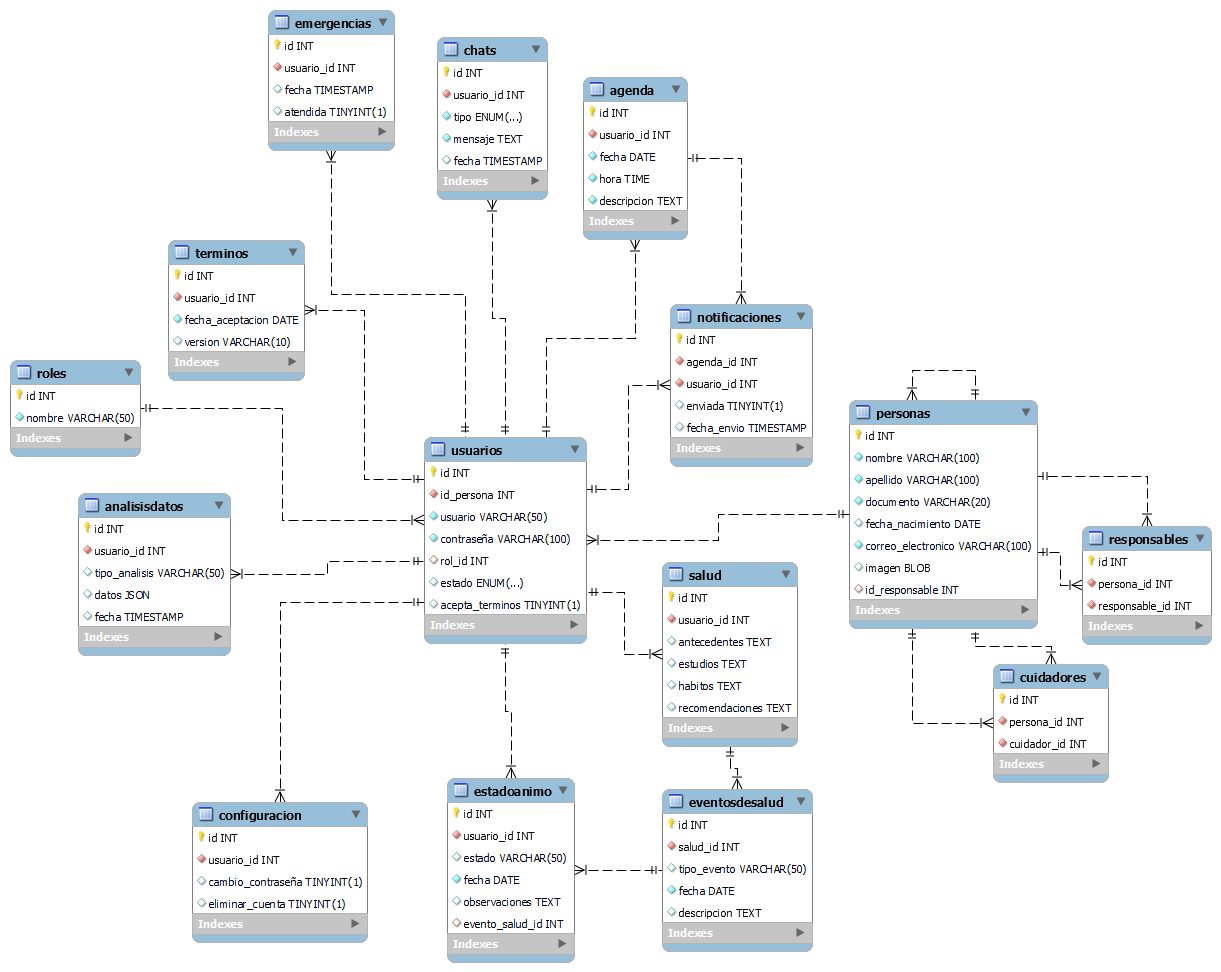
\includegraphics[width=1\textwidth]{Imagenes/DER.png}

    \newpage

% Metodología a Utilizar
    \section{Metodología a utilizar}
    \par La metodología que adoptaremos a lo largo del desarrollo del proyecto es la \textbf{Iterativa Incremental}. Resulta adecuada para el proyecto gracias a la flexibilidad y adaptabilidad que ofrece a lo largo del tiempo de vida del mismo. En ella descomponemos el desarrollo en ciclos donde se adicionan diferentes módulos y/o funcionalidades, obteniendo así las diferentes versiones.
    \par De esta forma el sistema se desarrolla poco a poco, permitiéndonos obtener un feedback continuo, responder a las posibles mejoras y reaccionar a los cambios en los requerimientos.
    \saltolinea
    \par\noindent 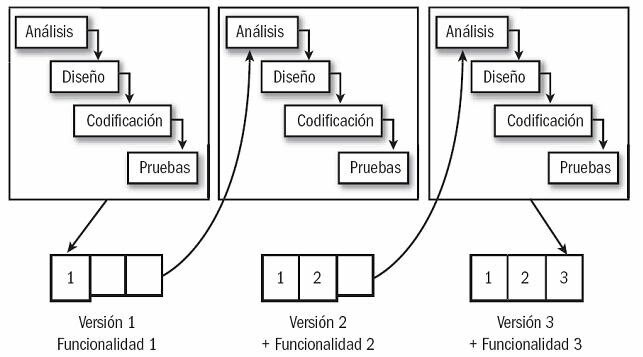
\includegraphics[width=1\textwidth]{Imagenes/IterativoIncremental.png}
    

    \newpage

% Tamaño del Sistema
    \section{Especificación funcional del sistema}
    \par En esta sección detallamos el \textbf{comportamiento funcional} de la aplicación: los módulos que la componen, las operaciones que cada uno habilita, las reglas de negocio que los gobiernan y las restricciones de acceso que se les aplican. Constituye la especificación de referencia del sistema y la base sobre la cual se realiza, en la sección siguiente, el \textit{Cálculo del tamaño del sistema}.
    \par La descripción avanza siguiendo el recorrido natural del usuario: comienza por el acceso a la aplicación (registro, validación de identidad, verificación de correo y recuperación de contraseña), continúa por el menú principal y las pantallas de perfil y configuración, y desarrolla luego los módulos de negocio propiamente dichos —personas a cargo, equipo de cuidado, agenda, salud y emergencia—. Cierra con las reglas de negocio que atraviesan a todos los módulos y con las limitaciones conocidas de la versión actual.
    \subsection{Iniciar Sesión}
    \par Los usuarios pueden acceder al sistema a través de la opción de \textit{``Iniciar sesión''} disponible en la primera pantalla de la aplicación, la cual también ofrece la opción de \textit{``Registrarse''}.
    \par Al seleccionar \textit{``Iniciar sesión''}, se mostrará la pantalla de autenticación. En esta, los usuarios deberán completar los campos:
    \begin{itemize}
        \item Email
        \item Contraseña
    \end{itemize}
    \par Estos datos deben coincidir con los proporcionados al momento de la creación de la cuenta. El identificador de acceso es el \textit{email} del usuario; si bien la implementación admite además el nombre de usuario, la pantalla de inicio de sesión solicita el email.
    \par Al presionar el botón \textit{``Ingresar''}, el sistema verificará la validez de la información ingresada. Si los datos son correctos, se permitirá el acceso al menú principal de la aplicación. Si alguno de los campos es incorrecto, se mostrará un mensaje de error debajo de los campos correspondientes, informando al usuario del problema e impidiendo el acceso.
    \par Adicionalmente, esta pantalla incluye un acceso a la recuperación de contraseña (\textit{``¿Olvidaste tu contraseña?''}), destinado al usuario que no recuerda su clave. El flujo se resuelve mediante el envío de un código de verificación al correo registrado en la cuenta y se detalla en la subsección \textit{Recuperación de contraseña}.
    \par Finalmente, para quienes aún no tengan una cuenta, se incluye el botón \textit{``Crear cuenta''}, acompañado del mensaje \textit{``¿Aún no tienes cuenta?''}. Al pulsarlo, el sistema redirigirá a la pantalla de registro. Una vez completado el registro con éxito, el usuario debe verificar su correo electrónico mediante un código (véase \textit{Verificación de correo electrónico}) y luego regresa de forma manual a esta pantalla de inicio de sesión para autenticarse; no se realiza un inicio de sesión automático tras el alta.
    \par Por otro lado, el inicio de sesión y el registro de un usuario son procesos separados. Esto significa que una persona puede estar registrada en el sistema sin haber creado un usuario y contraseña de acceso. Esto es posible porque la aplicación está diseñada para permitir que los datos de usuarios que no tienen los medios o capacidades para utilizarla sean ingresados a través de sus responsables o cuidadores. En estos casos, podría haber usuarios que no hayan iniciado sesión anteriormente, pero que deseen hacerlo por primera vez. En tal situación, el acceso a la creación de credenciales es \textit{manual}: la pantalla de inicio de sesión ofrece el enlace \textit{``Mi cuenta fue creada por otro''}, que conduce a la pantalla donde la persona puede crear sus credenciales de acceso (email y contraseña) por primera vez. No existe una redirección automática. Para evitar que un tercero se apropie del registro de otra persona, este flujo exige superar la \textbf{validación de identidad} mediante el documento del solicitante (véase la subsección \textit{Validación de identidad}).
    \subsection{ABM de Usuarios}
    \par Este módulo permite gestionar eficientemente a los usuarios mediante las siguientes acciones:
    \begin{itemize}
        \item \textbf{Alta de usuarios:} Registrar nuevos usuarios e ingresar sus datos personales.
        \item \textbf{Baja de usuarios:} La baja es \textbf{autogestionada por el propio titular} de la cuenta, quien puede solicitarla desde la pantalla de \textit{Configuración} (véase la subsección \textit{Configuración}). Se trata de una \textbf{baja lógica}: revoca el acceso del usuario al sistema sin suprimir su registro. El sistema no contempla un rol administrador ni la posibilidad de que un usuario dé de baja la cuenta de otro.
        \item \textbf{Modificación de datos:} Actualizar la información personal del usuario, tal como sus nombres o sus datos de contacto, desde la pantalla de \textit{Mi Perfil}. El \textbf{rol} de una persona no es un atributo del usuario sino de cada asignación de cuidado, y no admite modificación una vez creada (véase la subsección \textit{Reglas de negocio transversales}).
    \end{itemize}
    \par Consideraciones adicionales:
    \begin{itemize}
        \item No es posible crear un usuario si alguno de los campos obligatorios no ha sido completado. El formulario de registro exige, además de los datos personales y las credenciales (email y contraseña), el \textbf{teléfono} como campo obligatorio.
        \item Un usuario puede estar registrado solo una vez en el sistema, por lo que se debe validar que no exista.
        \item Es obligatorio que el usuario acepte los Términos y Condiciones para completar el registro; en caso de no aceptarlos, no se procesará la creación de la cuenta.
        \item Es obligatorio aportar una fotografía del documento de identidad y superar la \textbf{validación de identidad}: si los datos declarados no coinciden con los del documento, la cuenta no se crea (véase la subsección \textit{Validación de identidad}).
    \end{itemize}
    \par Una vez procesado correctamente el alta, la cuenta queda creada pero en estado \textit{pendiente de validación}: antes de poder acceder, el usuario debe confirmar su dirección de correo electrónico mediante un código de verificación. Por ello, tras completar el registro el sistema conduce al usuario a la pantalla de verificación del código, tal como se detalla en la subsección \textit{Verificación de correo electrónico}. El registro no realiza un inicio de sesión automático: una vez verificada la cuenta, el usuario debe ingresar sus credenciales de forma manual desde la pantalla de login para acceder al sistema.
    \subsection{Validación de identidad}
    \par Dado que la aplicación custodia información personal y de salud, el sistema debe asegurarse de que quien crea una cuenta \textbf{es efectivamente la persona que dice ser}, y no un tercero que se apropia de la identidad ajena para acceder a datos sensibles. A tal fin incorpora una \textbf{validación de identidad} basada en el \textbf{documento nacional de identidad} del solicitante, asistida por un componente de \textbf{inteligencia artificial} de reconocimiento de texto sobre imágenes.
    \par Es importante distinguir esta validación de la \textit{verificación de correo elec\-tró\-ni\-co} descrita en la subsección siguiente: aquella confirma que el solicitante \textbf{controla la casilla de correo} declarada; esta confirma que el solicitante \textbf{es el titular de los datos personales} declarados. Ambas son complementarias y ambas deben superarse para operar con una cuenta.
    \par La validación se exige en los \textbf{dos flujos en los que nace una credencial de acceso}:
    \begin{itemize}
        \item \textbf{Registro de una cuenta nueva:} cuando una persona se da de alta por sus propios medios y declara sus datos personales.
        \item \textbf{Reclamo de una persona ya registrada:} cuando una persona que fue cargada previamente en el sistema por un responsable o cuidador —y que por lo tanto existe sin credenciales— decide crear su acceso para administrar su propia información. Este flujo se inicia desde el enlace \textit{``Mi cuenta fue creada por otro''} de la pantalla de inicio de sesión (véase la subsección \textit{Iniciar Sesión}). La validación de identidad es aquí especialmente crítica, ya que impide que un tercero se apropie del registro de otra persona y acceda a su historial.
    \end{itemize}
    \par En cambio, el alta de una \textbf{persona a cargo} no requiere esta validación, puesto que no genera credenciales de acceso: quien la registra es un responsable o cuidador que ya validó su propia identidad, y la persona registrada podrá validar la suya más adelante, si alguna vez reclama su cuenta.
    \par El \textbf{funcionamiento} es el siguiente: el usuario aporta una \textbf{fotografía de su documento de identidad}. El sistema entrega esa imagen a un componente de inteligencia artificial que \textbf{extrae de ella el número de documento, el nombre y el apellido}. Luego \textbf{contrasta} esos valores contra los datos que el usuario declaró en el formulario. La comparación se realiza de forma tolerante a las diferencias de escritura habituales —no distingue mayúsculas de minúsculas ni considera los acentos—, de modo que una discrepancia meramente ortográfica no impida una validación legítima.
    \par Las \textbf{reglas de negocio} que rigen la validación son las siguientes:
    \begin{itemize}
        \item \textbf{Carácter obligatorio y bloqueante:} la validación es \textbf{condición necesaria} para completar tanto el registro como el reclamo de una cuenta. Si no se supera, la operación \textbf{no se concreta}: no se crea la cuenta ni las credenciales, y el usuario debe reintentar hasta lograr una validación exitosa.
        \item \textbf{Imagen requerida:} no es posible continuar sin aportar la imagen del documento; su ausencia se rechaza antes de invocar al componente de inteligencia artificial.
        \item \textbf{Coincidencia total:} la identidad se considera validada únicamente si \textbf{los tres datos} —número de documento, nombre y apellido— coinciden con los declarados. La coincidencia parcial no habilita la operación.
        \item \textbf{Fallas de lectura:} si la imagen resulta ilegible, si el componente no logra extraer los datos o si los extraídos no coinciden con los declarados, el sistema informa al usuario que no fue posible validar su identidad y lo orienta a reintentar con una fotografía nítida y legible, cuyos datos coincidan con su documento.
        \item \textbf{Indisponibilidad del servicio:} si el componente de inteligencia artificial no se encuentra disponible, el sistema lo comunica como una \textbf{falla temporal del servicio}, distinguiéndola de un rechazo de la identidad. En ningún caso la indisponibilidad habilita a omitir la validación.
        \item \textbf{No persistencia de la imagen:} la fotografía del documento se utiliza \textbf{exclusivamente} para esta comprobación y \textbf{no se almacena} en el sistema. Se procesa en el momento y se descarta; no queda registrada en la base de datos ni asociada al legajo de la persona.
        \item \textbf{Constancia de la validación:} superada la comprobación, la persona queda marcada como \textbf{de identidad validada}, dejándose asentada además la \textbf{fecha} en que ello ocurrió. Lo que se conserva es entonces el \textit{hecho} de la validación y su fecha, nunca la imagen que le dio origen.
    \end{itemize}
    \par El componente de inteligencia artificial empleado se despliega de forma \textbf{self-hosted}, bajo control del propio sistema, de modo que la imagen del documento \textbf{no se remite a ningún proveedor tercero externo}. Este criterio es el mismo adoptado para el \textit{Resumen diario} (véanse las subsecciones \textit{Resumen diario de la persona a cargo} y \textit{Riesgo 2 - Integración de IA}).
    \subsection{Verificación de correo electrónico}
    \par Como parte del proceso de alta de una cuenta con credenciales propias, el sistema incorpora una \textbf{verificación del correo electrónico} mediante un código de un solo uso. Su finalidad es confirmar que la dirección de correo declarada pertenece efectivamente a quien se registra, condición necesaria para habilitar el acceso al sistema. Esta verificación aplica al \textbf{alta de la cuenta}; el cambio de email posterior y la recuperación de contraseña son flujos separados que, si bien comparten la idea de un código temporal, no forman parte del alcance de esta sección.
    \par El flujo funcional es el siguiente:
    \begin{itemize}
        \item \textbf{Generación y envío del código:} al completarse el registro, el sistema genera automáticamente un \textbf{código de verificación de seis dígitos} y lo envía por correo electrónico a la dirección registrada. El envío efectivo de este y de los demás correos de la aplicación se realiza a través de \textbf{Elastic Email}, servicio externo utilizado como proveedor de envío de correo electrónico transaccional. La cuenta queda en estado \textit{pendiente de validación} hasta que el usuario confirme dicho código.
        \item \textbf{Vigencia del código:} el código tiene una validez de \textbf{diez minutos} desde su generación. Transcurrido ese plazo, expira y deja de ser válido para confirmar la cuenta.
        \item \textbf{Confirmación:} cuando el usuario ingresa correctamente el código dentro de su plazo de vigencia, la cuenta pasa a estado \textit{activo} y el usuario queda habilitado para iniciar sesión con sus credenciales.
        \item \textbf{Intentos de verificación:} el usuario dispone de un máximo de \textbf{cinco intentos} para ingresar el código correcto. Si agota los cinco intentos sin acertar, el código queda invalidado y deberá solicitar el envío de uno nuevo para poder continuar.
        \item \textbf{Reenvío del código:} el usuario puede solicitar que se le reenvíe el código, por ejemplo si no lo recibió o si ya expiró. Para evitar abusos, existe un tiempo mínimo de espera de \textbf{sesenta segundos} entre reenvíos y un máximo de \textbf{cinco envíos por hora}. Cada vez que se genera un código nuevo, cualquier código anterior pendiente queda invalidado, de modo que \textbf{solo existe un código válido vigente a la vez}.
        \item \textbf{Bloqueo de acceso:} mientras la cuenta permanezca en estado \textit{pendiente de validación}, el usuario \textbf{no puede iniciar sesión}. Al intentarlo, el sistema le informa que debe verificar su correo electrónico antes de poder ingresar.
        \item \textbf{Privacidad ante reenvíos:} cuando se solicita el reenvío de un código para una dirección de correo que no está registrada en el sistema, la respuesta es la misma que si la dirección existiera. De este modo, el sistema no revela si un correo se encuentra o no registrado, resguardando la privacidad de las cuentas.
    \end{itemize}
    \par En consecuencia, la habilitación efectiva de una cuenta recién creada depende de que su titular confirme el código recibido. Esta regla complementa lo descrito en las secciones \textit{Iniciar Sesión} y \textit{ABM de Usuarios}: el alta crea la cuenta, pero el acceso queda condicionado a la verificación del correo.
    \par Desde la perspectiva del usuario, la aplicación acompaña este flujo del siguiente modo:
    \begin{itemize}
        \item \textbf{Ingreso a la verificación tras el registro:} al completar el registro con éxito, en lugar de conducir directamente al inicio de sesión, el sistema lleva al usuario a una pantalla de \textbf{verificación de código}. Allí se le informa que se envió un código de seis dígitos a su correo electrónico y que debe ingresarlo para activar la cuenta.
        \item \textbf{Ingreso del código:} el usuario introduce en esa pantalla el código de seis dígitos recibido. Si el código es incorrecto, expiró o se agotaron los intentos disponibles, el sistema muestra el mensaje correspondiente, según las reglas de negocio descritas más arriba. Si el código es correcto, la cuenta queda activada y el sistema conduce al usuario a la pantalla de inicio de sesión. La verificación \textbf{no inicia sesión automáticamente}: una vez activada la cuenta, el usuario debe autenticarse con sus credenciales.
        \item \textbf{Reenvío desde la interfaz:} desde la misma pantalla, el usuario puede solicitar el reenvío del código si no lo recibió o si venció. Cuando el pedido ocurre antes de cumplirse el tiempo mínimo de espera, o cuando se superó el máximo de envíos por hora, el sistema se lo informa y, para orientarlo, \textbf{deshabilita el botón de reenvío mostrando una cuenta regresiva} hasta que sea posible solicitarlo nuevamente.
        \item \textbf{Reingreso con cuenta pendiente de validación:} si un usuario cuya cuenta aún no fue verificada intenta iniciar sesión (por ejemplo, porque cerró la aplicación antes de completar la verificación y regresa más tarde), el sistema no le permite el acceso y lo \textbf{redirige a la pantalla de verificación de código}, en lugar de presentarle un error genérico de credenciales. De este modo, el usuario puede retomar la activación de su cuenta desde donde la dejó.
    \end{itemize}
    \par Los mensajes que se muestran ante un código incorrecto, expirado o con intentos agotados, así como los avisos de espera y de límite de envíos, son los mismos definidos por las reglas de negocio del backend descritas en esta subsección; la interfaz se limita a presentarlos al usuario en el momento adecuado. La experiencia end-to-end resultante ---generación y envío del código, ingreso y confirmación, reenvío controlado y bloqueo del acceso hasta la validación--- constituye el comportamiento definido del sistema para el alta de cuentas con credenciales propias.
    \subsection{Recuperación de contraseña}
    \par Cuando un usuario no recuerda su contraseña, el sistema le permite \textbf{restablecerla} sin intervención de un administrador, a través de un flujo iniciado desde el enlace \textit{``¿Olvidaste tu contraseña?''} de la pantalla de inicio de sesión. El mecanismo reutiliza el mismo esquema de \textbf{código de verificación de un solo uso} empleado en el alta de la cuenta (véase la subsección \textit{Verificación de correo electrónico}), de modo que el sistema mantiene un único mecanismo de códigos para todos los flujos que requieren confirmar la titularidad de una dirección de correo. No se utilizan enlaces de restablecimiento embebidos en el correo.
    \par El flujo consta de \textbf{dos etapas}:
    \begin{itemize}
        \item \textbf{Solicitud del restablecimiento:} el usuario indica la dirección de correo electrónico asociada a su cuenta. El sistema genera un \textbf{código de seis dígitos} y lo envía a esa dirección.
        \item \textbf{Confirmación y cambio:} el usuario ingresa el código recibido junto con la \textbf{nueva contraseña}. Si el código es válido y no expiró, la contraseña se reemplaza y el usuario queda habilitado para iniciar sesión con ella.
    \end{itemize}
    \par Las \textbf{reglas de negocio} que rigen el flujo son las siguientes:
    \begin{itemize}
        \item \textbf{Parámetros del código:} el código tiene una vigencia de \textbf{diez minutos}, admite un máximo de \textbf{cinco intentos} de ingreso, exige una espera mínima de \textbf{sesenta segundos} entre reenvíos y un máximo de \textbf{cinco envíos por hora}. Cada nuevo código invalida al anterior, de modo que \textbf{solo existe un código válido vigente a la vez}. Estos parámetros son los mismos que rigen la verificación de correo del alta.
        \item \textbf{Independencia entre flujos:} los códigos se emiten \textbf{diferenciados por finalidad}. Un código emitido para recuperar la contraseña no puede utilizarse para verificar el alta de la cuenta, ni a la inversa.
        \item \textbf{Cuenta habilitada:} únicamente puede restablecer su contraseña un usuario cuya cuenta se encuentre en estado \textit{activo}. Una cuenta \textit{pendiente de validación} debe completar primero la verificación de su correo electrónico.
        \item \textbf{Privacidad ante la solicitud:} si la dirección indicada no corresponde a ninguna cuenta registrada, el sistema responde exactamente igual que si existiera, sin enviar correo alguno. De este modo \textbf{no se revela si un correo se encuentra registrado}, resguardando la privacidad de las cuentas.
        \item \textbf{Validación de la nueva contraseña:} la contraseña propuesta debe cumplir las mismas exigencias de complejidad que se aplican en el alta de la cuenta.
        \item \textbf{Cierre de sesiones activas:} al restablecerse la contraseña, el sistema \textbf{revoca todas las sesiones vigentes} del usuario en cualquier dispositivo. Así, si un tercero hubiera obtenido acceso a la cuenta, el restablecimiento lo expulsa de inmediato y el legítimo titular debe autenticarse nuevamente con su nueva clave.
    \end{itemize}
    \par Completado el restablecimiento, el sistema conduce al usuario a la pantalla de inicio de sesión. El flujo \textbf{no inicia sesión automáticamente}: el usuario debe autenticarse con su nueva contraseña.
    \subsection{Menú Principal}
    \par La pantalla del menú principal es la interfaz central del sistema, desde la cual los usuarios pueden acceder a las diferentes funcionalidades de la aplicación. Esta será la pantalla predeterminada a la que se regresará cada vez que se presione el ícono de la aplicación en las distintas pantallas donde esté disponible.
    \par En la parte superior, el menú principal presenta un \textbf{encabezado} con el saludo personalizado al usuario y un \textbf{acceso a la Configuración}, representado por la imagen de perfil del usuario. Desde la pantalla de \textit{Configuración} se accede, a su vez, a \textit{Mi Perfil}, donde el usuario visualiza y modifica sus datos personales (véanse las secciones \textit{Mi Perfil} y \textit{Configuración}). Todas las pantallas secundarias cuentan con un botón que permite regresar fácilmente al menú principal.
    \par Debajo del encabezado, la pantalla presenta el \textbf{selector de persona a cargo} y el \textbf{acceso al Resumen diario} de la persona de contexto (véase la sección \textit{Resumen diario de la persona a cargo}).
    \par A continuación, el menú principal ofrece los accesos a las funcionalidades clave del sistema, cada uno de ellos enlazado a su respectiva sección:
    \begin{itemize}
        \item \textbf{Calendario:} acceso al módulo de agenda (véase \textit{Gestión de Agenda}).
        \item \textbf{Equipo de cuidado:} acceso a la gestión de responsables y cuidadores (véanse \textit{ABM de Responsables} y \textit{ABM de Cuidadores}).
        \item \textbf{Personas a cargo:} acceso al listado de personas bajo cuidado y a las invitaciones recibidas (véase \textit{ABM de Personas a Cargo}).
        \item \textbf{Salud:} acceso al módulo \textit{Salud} (véase \textit{Gestión de Salud}).
        \item \textbf{Emergencia:} acceso destacado y siempre visible al aviso de emergencia (véase \textit{Emergencia}).
    \end{itemize}
    \par Los cuatro primeros accesos se disponen en una grilla, mientras que el acceso a \textit{Emergencia} se presenta de forma diferenciada y permanentemente visible, dada su criticidad. Al presionar cualquiera de ellos, el usuario será dirigido a la pantalla correspondiente, permitiendo un acceso rápido y eficiente a las diversas funciones de la aplicación. El acceso a \textit{Salud} incorpora además un indicador visual que refleja el último estado de ánimo registrado de la persona de contexto, de modo que el bienestar emocional tenga presencia en el menú principal sin necesidad de ingresar a la sección de salud.
    \par El \textbf{selector de persona a cargo} define la persona de contexto que el usuario está visualizando. Esta selección actúa como un filtro global que condiciona la información mostrada en las pantallas secundarias (Calendario, Equipo de cuidado, Personas a cargo, Salud, Emergencia y Resumen diario), de modo que un responsable que cuida a más de una persona pueda alternar entre ellas y ver en cada caso la información correspondiente. El menú muestra de forma visible la persona seleccionada y permite cambiarla sin abandonar el flujo principal; la selección persiste durante la sesión. Si el usuario tiene una única persona a cargo, esta se muestra sin opción de cambio, y si no tiene ninguna se le indica que debe agregar una primero. La persona de contexto también determina a quién corresponde la alerta del módulo de emergencia. Cuando el propio usuario es la persona de contexto seleccionada, accede a todas las funcionalidades de registro sobre sus propios datos sin restricción de permisos de equipo: el propio usuario siempre puede registrar sobre su propio perfil sin requerir pertenecer a un equipo de cuidado.
    \subsection{Mi Perfil}
    \par El módulo \textit{Mi perfil} permite a los usuarios visualizar y editar su información personal. La pantalla principal del perfil incluye los datos personales del usuario. Cada uno de los campos cuenta con un ícono de edición, lo que permite al usuario actualizar sus datos de manera sencilla. La interfaz es clara y accesible, mostrando un ícono de perfil en la parte superior y un botón de navegación para volver a la pantalla anterior. Además, la información está organizada de manera ordenada, con botones para modificar cada uno de los campos de manera independiente.
    \subsection{Configuración}
    \par El módulo de \textit{Configuración} brinda a los usuarios diversas opciones para gestionar su cuenta y mantener la seguridad de su información.
    \begin{itemize}
        \item \textbf{Términos y condiciones:} Permite acceder a una pantalla que muestra los términos y condiciones aceptados al crear la cuenta. Los usuarios pueden revisarlos en cualquier momento y regresar al menú anterior mediante un botón de navegación.
        \item \textbf{Seguridad y privacidad:} Incluye dos opciones.
        \item \textbf{Cambio de contraseña:} Permite al usuario con sesión iniciada modificar su contraseña. A diferencia del flujo de \textit{Recuperación de contraseña} —pensado para quien no puede acceder a su cuenta y por ello se apoya en un código enviado por correo—, aquí la identidad del usuario ya está acreditada por la sesión activa, de modo que el sistema solicita la \textbf{contraseña actual} junto con la nueva. La contraseña propuesta debe cumplir las mismas exigencias de complejidad que rigen en el alta de la cuenta.
        \item \textbf{Eliminación de cuenta:} Ofrece al titular la opción de eliminar su propia cuenta. Antes de proceder, se solicita confirmación mediante un mensaje de advertencia; si el usuario cancela, no se realiza cambio alguno. Al confirmar, la cuenta pasa a estado \textit{eliminada}: el usuario \textbf{pierde el acceso al sistema} y se \textbf{desactivan todos sus dispositivos registrados}, de modo que deja de recibir notificaciones. Se trata de una \textbf{baja lógica}: el registro de la persona se conserva, ya que puede integrar el equipo de cuidado de terceros y su información forma parte del historial de otras personas del sistema. La supresión definitiva de los datos personales puede solicitarse por los canales previstos en la \textit{Política de privacidad}, conforme a los derechos reconocidos por la normativa de protección de datos.
        \item \textbf{Cerrar sesión:} Permite al usuario cerrar la sesión y regresar automáticamente a la pantalla de inicio.
    \end{itemize}
    \subsection{ABM de Responsables}
    \par El módulo de \textit{Alta, Baja y Modificación (ABM) de Responsables} permite gestionar a los usuarios que tienen asociados a otros usuarios, conocidos como responsables. Ellos poseen permisos adicionales que les permiten modificar los datos personales de los usuarios y realizar otras acciones específicas.
    \par Desde la pantalla del menú principal, al presionar el botón \textit{``Equipo de cuidado''}, los usuarios accederán a una interfaz que muestra todos los responsables y cuidadores asociados. Este módulo permite gestionar los permisos y accesos de cada miembro del equipo de cuidado del usuario a través de las siguientes funcionalidades:
    \begin{itemize}
        \item \textbf{Alta de responsables:} Facilita el registro de nuevos responsables en el equipo. Esta acción es independiente del alta de cuidadores y asigna explícitamente el rol \textit{Responsable}. Por defecto, un responsable recibe \textbf{todos los permisos del catálogo activados}, ajustables posteriormente. Toda alta de miembro nace en estado \textit{pendiente}: la persona invitada debe aceptarla o rechazarla desde su pantalla \textit{``Personas a cargo''} (sección \textit{``Invitaciones de cuidado''}) antes de integrarse efectivamente al equipo (véase la regla transversal \textit{Flujo de invitación y aceptación de miembros}). El origen autoritativo de los permisos por defecto es el backend; los valores aplicados en el frontend son provisionales.
        \item \textbf{Baja de responsables:} Permite eliminar a un responsable del equipo de cuidado. Esta acción revocará su acceso y permisos en el sistema. Se trata de una baja lógica: el miembro permanece visible en la sección \textit{``Recientemente eliminados''} durante la ventana de reactivación.
        \item \textbf{Modificación de responsables:} Ofrece la opción de actualizar los permisos de cada miembro del equipo. Desde la pantalla de gestión, el usuario podrá acceder a los detalles del miembro seleccionado y realizar las modificaciones necesarias.
    \end{itemize}
    \par La pantalla \textit{``Equipo de cuidado''} se organiza en secciones: el listado de miembros activos del equipo, la sección \textit{``Solicitudes pendientes''} (invitaciones aún no aceptadas por sus destinatarios) y la sección \textit{``Recientemente eliminados''} (miembros dados de baja que todavía se encuentran dentro de la ventana de reactivación, identificados con el texto \textit{“Vence en N días”}). El acceso a estas funcionalidades está condicionado por las siguientes reglas:
    \begin{itemize}
        \item \textbf{Ver el equipo:} cualquier miembro activo del equipo de cuidado puede consultar el listado de miembros; el propio usuario también accede en su contexto propio.
        \item \textbf{Administrar el equipo} (agregar un miembro, ver el detalle de un miembro y reactivar miembros eliminados): requiere contar con el permiso \textit{Administrar equipo de cuidado} o encontrarse en contexto propio.
        \item \textbf{Ver la sección \textit{``Solicitudes pendientes''}:} está reservada exclusivamente al responsable activo de la persona a cargo.
        \item \textbf{Otorgar el permiso \textit{Administrar equipo de cuidado}:} solo un responsable puede conceder este permiso a otro miembro del equipo.
    \end{itemize}
    \par No existe la posibilidad de cambiar el rol de un miembro una vez creada la asignación; no obstante, pueden asignarse todos los permisos del catálogo a cualquier rol. Para cambiar el rol de un miembro se debe dar de baja la asignación y volver a invitarlo con el nuevo rol.
    \par Desde esta interfaz, los usuarios podrán tener un registro claro de quienes componen su equipo de cuidado, así como gestionar eficazmente sus accesos y permisos.
    \subsection{ABM de Cuidadores}
    \par Los cuidadores son personas encargadas de realizar diversas actividades de cuidado para el usuario. Por esta razón, es fundamental que tengan acceso a ciertas funcionalidades e información del usuario. Desde la pantalla del menú principal, al presionar el botón \textit{``Equipo de cuidado''}, los usuarios accederán a una interfaz que muestra todos los responsables y cuidadores asociados. Este módulo permite gestionar los permisos y accesos de cada miembro del equipo de cuidado a través de las siguientes funcionalidades:
    \begin{itemize}
        \item \textbf{Alta de cuidadores:} Esta opción permite a los usuarios agregar nuevos cuidadores a su equipo, mediante una acción diferenciada del alta de responsables. El alta de cuidador asigna explícitamente el rol \textit{Cuidador} y, una vez registrado, se le asignan permisos iniciales más restringidos que los de un responsable: por defecto quedan activados únicamente los permisos \textit{Ver ficha de salud} y \textit{Gestionar agenda}, y el resto permanece desactivado. Estos valores son ajustables posteriormente y su origen autoritativo es el backend (el frontend aplica defaults provisionales). Al igual que el alta de responsables, toda alta de cuidador nace en estado \textit{pendiente} y requiere que la persona invitada la acepte o rechace desde su pantalla \textit{``Personas a cargo''} (sección \textit{``Invitaciones de cuidado''}) antes de integrarse al equipo. El rol del miembro lo determina la acción de alta elegida y no puede modificarse una vez creada la asignación.
        \item \textbf{Baja de cuidadores:} Esta funcionalidad permite a los usuarios eliminar a un cuidador del equipo. Al realizar esta acción, se revocará de inmediato su acceso y permisos en el sistema, garantizando que solo los cuidadores activos puedan interactuar con la información del usuario.
        \item \textbf{Modificación de cuidadores:} A través de esta opción, los usuarios pueden actualizar los permisos de los cuidadores existentes. Desde la interfaz, podrán acceder a los detalles de cada cuidador y realizar los cambios necesarios de manera sencilla y eficiente.
    \end{itemize}
    \par Este módulo facilita la gestión del equipo de cuidado, asegurando que los usuarios puedan agregar, eliminar o modificar cuidadores según sus necesidades.
    \subsubsection{Catálogo de permisos del sistema}
    \par El control de acceso basado en roles (RBAC) se apoya en un catálogo cerrado de permisos que se asignan a cada miembro del equipo de cuidado. El sistema define exactamente \textbf{siete} permisos, cuya combinación determina las acciones que un responsable o cuidador puede realizar sobre la persona a cargo:
    \begin{itemize}
        \item \textbf{Ver ficha de salud:} consultar la información de salud de la persona a cargo.
        \item \textbf{Editar ficha de salud:} modificar la ficha de salud de la persona a cargo.
        \item \textbf{Gestionar agenda:} crear, modificar y eliminar eventos y recordatorios de la agenda.
        \item \textbf{Registrar eventos de salud:} dar de alta eventos de salud (consultas, hospitalizaciones, etc.).
        \item \textbf{Registrar hábitos de vida:} dar de alta y mantener los hábitos de vida.
        \item \textbf{Activar emergencia:} activar el botón de emergencia para la persona a cargo.
        \item \textbf{Administrar equipo de cuidado:} gestionar los miembros del equipo, sus roles y sus permisos.
    \end{itemize}
    \par Los \textbf{permisos por defecto} que recibe cada miembro al ser dado de alta dependen de su rol: un \textit{Responsable} recibe los siete permisos activados, mientras que un \textit{Cuidador} recibe activados únicamente \textit{Ver ficha de salud} y \textit{Gestionar agenda}, quedando el resto desactivado. El origen autoritativo de estos valores por defecto es el \textbf{backend}; la configuración aplicada en el frontend es provisional. El permiso \textit{Administrar equipo de cuidado} solo puede ser otorgado a un miembro por un responsable.
    \par Cabe recordar que cuando el propio usuario es la persona de contexto seleccionada, accede a todas las funcionalidades de registro sobre sus propios datos sin restricción de permisos de equipo (véase la sección \textit{Menú Principal} y la regla transversal de contexto propio).
    \subsection{ABM de Personas a Cargo}
    \par Desde el menú principal, los usuarios pueden acceder al módulo \textit{ABM de Personas a Cargo} mediante el botón \textit{“Personas a cargo”}. Este módulo permite gestionar a los responsables y cuidadores en los que forma parte del equipo de cuidado de otros usuarios, facilitando así el alta, baja y modificación de los datos de las personas a su cargo.
    \par Al ingresar, se mostrará un listado de todas las personas que están bajo la responsabilidad del usuario, diferenciando entre las secciones correspondientes a responsables y cuidadores. Desde esta interfaz, los usuarios pueden acceder a los datos y funcionalidades de las personas a su cargo. El listado incluye también las asignaciones que han sido eliminadas (estado \textit{inactiva}) durante la ventana de reactivación de \textbf{30 días} posteriores a la eliminación; estas asignaciones se presentan con un \textbf{indicador visual de estado “eliminada”} que las distingue de las activas y muestran el texto \textit{“Vence en N días”}, donde N es la cantidad de días restantes de la ventana de reactivación. Este comportamiento de mostrar \textit{“Vence en N días”} sobre los registros eliminados es el definido tanto para \textit{Personas a cargo} como para \textit{Equipo de cuidado} (sección \textit{``Recientemente eliminados''}).
    \par La pantalla de \textit{Personas a cargo} incluye además la sección \textit{``Invitaciones de cuidado''}, donde el usuario visualiza las invitaciones que ha recibido para integrarse al equipo de cuidado de otra persona (ya sea como responsable o como cuidador) y que aún se encuentran en estado \textit{pendiente}. Desde allí puede \textbf{aceptar} o \textbf{rechazar} cada invitación: al aceptarla, la asignación pasa a estado activo y la persona a cargo se incorpora a su listado; al rechazarla, la invitación se descarta. Ninguna asignación se vuelve efectiva hasta que el destinatario la acepta (véase la regla transversal \textit{Flujo de invitación y aceptación de miembros}).
    \par Las funcionalidades disponibles incluyen:
    \begin{itemize}
        \item \textbf{Modificar datos:} Permite actualizar la información de la persona a cargo. Esta acción está reservada a los \textit{responsables}: los cuidadores no pueden editar los datos de la persona a cargo, restricción que impone el backend. La modificación se realiza exclusivamente desde la \textbf{pantalla de detalle} de la persona a cargo, y no desde el formulario de alta, que solo permite crear nuevos registros.
        \item \textbf{Eliminar:} Ofrece la opción de eliminar a una persona del equipo de cuidado, revocando su acceso y cualquier funcionalidad asociada. Al igual que la modificación, esta acción está reservada a los \textit{responsables}. La eliminación es una \textbf{baja lógica}: la asignación pasa a estado \textit{inactiva} y conserva su trazabilidad, permaneciendo visible en el listado durante la ventana de reactivación.
        \item \textbf{Reactivar:} Permite restaurar una asignación eliminada dentro de la ventana de \textbf{30 días} posteriores a la baja. Al tocar una asignación inactiva, el comportamiento depende del rol del usuario en esa asignación: si el usuario es \textit{Responsable}, se muestra un diálogo de confirmación con el texto \textit{“¿Desea reactivar esta asignación?”} y, al confirmar, la asignación vuelve al estado activo; si el usuario es \textit{Cuidador}, la acción no produce ningún efecto. Transcurridos los 30 días la reactivación deja de estar disponible. Tanto la validación del plazo de 30 días como la recuperación de la lista de asignaciones eliminadas reactivables las realiza el \textbf{frontend}, a fin de no duplicar la lógica de negocio.
    \end{itemize}
    \par Además, este módulo facilita la creación de cuentas para personas que no cuentan con los medios o habilidades necesarias para usar la aplicación. Este proceso es esencial para llevar un registro de su estado de salud y actividades.
    \par Para crear una cuenta, se presentará un campo inicial donde se consultará si la cuenta será para el usuario que está realizando el registro o si se están ingresando datos para otra persona. Esta opción es crucial, dado que la aplicación está diseñada para aquellos que cuidan a otros que, en muchos casos, no pueden utilizar un celular debido a su condición.
    \par Al seleccionar la opción de registro para otra persona, se deberán completar los siguientes campos:
    \begin{itemize}
        \item Nombre
        \item Apellido
        \item Documento
        \item Fecha de nacimiento
        \item Correo electrónico
        \item Teléfono (opcional)
        \item Imagen
    \end{itemize}
    \par Estos mismos campos, incluido el \textbf{teléfono} como dato opcional, son los que pueden editarse posteriormente desde la pantalla de detalle de la persona a cargo.
    \par Una vez que se hayan completado correctamente todos los campos y superadas las validaciones correspondientes, el usuario deberá aceptar los \textit{“Términos y condiciones”} marcando la casilla correspondiente. Finalmente, debe presionar el botón \textit{“Crear cuenta”} para registrar el alta de la misma.
    \subsection{Gestión de Agenda}
    \par Una de las funcionalidades principales del sistema es la \textit{Gestión de Agenda}, donde se registran actividades, eventos y recordatorios (por ejemplo, de medicamentos o controles) que el usuario o su equipo considere relevante planificar. Desde la pantalla del menú principal, los usuarios pueden acceder a esta función.
    \par Los eventos de agenda son \textbf{registros simples de planificación temporal}. Por diseño, no admiten notas ni información adicional asociada: se evita deliberadamente atar información clínica o relevante a un evento de calendario que puede no llegar a ocurrir. La información enriquecible (notas, observaciones y datos clínicos) se concentra en el \textit{Evento de Salud} que estos eventos pueden originar (véase la sección \textit{Gestión de Salud}).
    \par Cada evento de agenda se compone de un \textbf{título}, una \textbf{descripción} opcional, un \textbf{tipo de evento} (seleccionado del catálogo \textit{TipoEvento}), una \textbf{fecha y hora de inicio} y una \textbf{duración} expresada en minutos. De manera opcional puede definirse una \textbf{anticipación de recordatorio}, también expresada en minutos: se trata de un \textit{offset} que indica cuántos minutos antes del inicio del evento se disparará la notificación, y no constituye una entidad independiente sino un atributo del propio evento.
    \par En la pantalla de gestión de agenda se presentará un listado de todas las notificaciones agendadas, cada una de las cuales mostrará:
    \begin{itemize}
        \item Fecha
        \item Hora
        \item Tipo de evento
        \item Descripción
    \end{itemize}
    \par Cada ítem del listado funcionará como una notificación de celular. La vinculación con Google Calendar (visualización de los registros en el calendario de Google) queda reservada a futuro como integración con servicios de terceros.
    \par Además, los ítems del listado pueden ser modificados o eliminados únicamente si la fecha y hora de la actividad aún no han transcurrido. Esto asegura que los usuarios mantengan control sobre su agenda.
    \par Al crear un evento de agenda, el usuario selecciona su \textbf{tipo} a partir del catálogo común \textit{TipoEvento}, compartido por los módulos de \textit{Agenda} y \textit{Salud}. Cada tipo posee un atributo \textbf{\textit{agendable}} que indica si puede utilizarse para crear un evento de agenda, de modo que el selector de la agenda ofrece únicamente los tipos marcados como agendables. Así, un evento de agenda y el evento de salud que eventualmente origine quedan clasificados bajo la misma categoría (véase la sección \textit{Gestión de Eventos}).
    \par Los eventos de agenda admiten \textbf{recurrencia}: pueden programarse repeticiones con frecuencia \textit{Diaria}, \textit{Semanal} o \textit{Mensual}, configurando el \textbf{intervalo} de repetición y, de forma opcional, una \textbf{fecha de fin}. Un evento sin recurrencia constituye una ocurrencia única. Sobre una serie recurrente es posible \textbf{cancelar una ocurrencia individual} sin afectar al resto de las repeticiones de la serie.
    \par Cada evento de agenda incluye además la opción \textit{“Generar evento de salud”}, \textbf{activada por defecto}. Cuando esta opción está activa, al producirse una ocurrencia del evento de agenda el sistema genera de forma automática un \textit{Evento de Salud} asociado en el módulo \textit{Salud}, heredando el mismo \textit{TipoEvento} y la fecha de la ocurrencia. Esta generación sigue el patrón de \textbf{puesta al día en la lectura} (\textit{catch-up on read}): los eventos de salud \textbf{no} se pre-generan para las ocurrencias futuras de una serie recurrente, sino que el sistema crea los eventos de salud pendientes de la ventana en el momento en que el usuario abre la agenda, considerando únicamente las ocurrencias ya transcurridas. El \textit{Evento de Salud} generado queda \textbf{vinculado al evento de agenda que lo originó y a la fecha de ocurrencia específica} mediante el atributo \textit{fechaOcurrenciaEventoAgenda}, lo que permite al usuario enriquecerlo posteriormente con notas y observaciones. Este vínculo es \textbf{meramente informativo} (se muestra como una insignia en la interfaz) y no ata el ciclo de vida del evento de salud al de la agenda: el usuario puede \textbf{eliminar libremente} el evento de salud generado y la agenda \textbf{no lo vuelve a crear}, ya que la puesta al día considera cada ocurrencia una sola vez. De este modo, el \textit{Evento de Salud} funciona como el registro persistente y enriquecible del historial, mientras el historial de salud se mantiene basado en hechos efectivamente ocurridos y no en planificación. Esto resuelve la dualidad entre planificación y registro: el evento de agenda representa la planificación, y el evento de salud, el registro efectivo.
    \par En cuanto a los recordatorios, se implementan como \textbf{notificaciones locales} programadas en el dispositivo del usuario que crea el evento. Esto significa que el recordatorio se dispara en ese dispositivo, y no en los del resto del equipo de cuidado: la notificación de un evento de agenda a los demás cuidadores o responsables designados queda reservada para una iteración posterior (véase la sección \textit{Limitaciones conocidas del MVP}). Este criterio se distingue del adoptado para el módulo de \textit{Emergencia}, cuyo aviso sí se emite desde el servidor hacia los dispositivos de todo el equipo.
    \par El acceso a la agenda sobre una persona a cargo distingue entre lectura y escritura. Las operaciones de \textbf{escritura} (crear, modificar o eliminar un evento y cancelar una ocurrencia) requieren pertenecer al equipo de cuidado de la persona con el permiso \textit{Gestionar agenda}, o bien encontrarse en contexto propio. Las operaciones de \textbf{lectura} (consultar el calendario) solo requieren pertenecer al equipo de cuidado de la persona mediante una asignación activa, o encontrarse en contexto propio, sin necesidad del permiso \textit{Gestionar agenda}. En todos los casos, el propio usuario siempre puede gestionar su propia agenda sin requerir pertenecer a un equipo de cuidado ni contar con permisos asignados.
    \subsection{Emergencia}
    \par El botón de \textit{Emergencia} es una funcionalidad esencial que permite al usuario solicitar ayuda de manera rápida y eficiente. Desde el menú principal de la aplicación, el usuario puede presionar el botón designado como \textit{``Emergencia''}.
    \par Al activar este botón se genera una notificación instantánea destinada a los miembros del equipo de la persona, incluidos responsables y cuidadores, que informa que el usuario está solicitando asistencia inmediata.
    \par La notificación incluirá información relevante, como la identificación del usuario que ha activado la emergencia y de la persona de contexto a la que corresponde la alerta, lo que permitirá a los miembros del equipo actuar con rapidez y eficacia. Además, se garantizará que la comunicación sea clara, para que los responsables y cuidadores comprendan la urgencia de la situación y puedan responder de acuerdo a la necesidad del usuario.
    \par El aviso de emergencia se materializa mediante \textbf{notificaciones push} emitidas por el servidor y entregadas a los dispositivos de los miembros del equipo de cuidado. A tal fin, cada dispositivo queda \textbf{registrado} contra la cuenta del usuario, de modo que el sistema conoce a qué destinos debe dirigir el aviso. Al activarse una emergencia, el servidor determina el conjunto de destinatarios —los miembros activos del equipo de cuidado de la persona de contexto— y remite el aviso a todos sus dispositivos registrados. Si alguno de esos registros dejó de ser válido (por ejemplo, porque el usuario desinstaló la aplicación o cerró sesión en ese dispositivo), el sistema lo detecta y lo \textbf{depura automáticamente}, evitando acumular destinos inutilizables.
    \par De este modo, y a diferencia de las notificaciones de la agenda —que se programan localmente en el dispositivo de quien crea el evento—, el aviso de emergencia \textbf{alcanza efectivamente a los demás miembros del equipo} aunque no tengan la aplicación abierta.
    \par Esta función está diseñada para ofrecer tranquilidad tanto al usuario como a su equipo, asegurando la disponibilidad de ayuda en momentos críticos.
    \subsection{Gestión de Salud}
    \par El módulo \textit{``Salud''} ofrece a los usuarios un espacio personal para gestionar su historial médico de forma integral. En esta sección, los usuarios pueden registrar y consultar una amplia variedad de información relacionada con su salud, incluyendo:
    \begin{itemize}
        \item \textbf{Hábitos de vida:} Permite llevar un registro detallado de hábitos como alimentación, ejercicio, sueño y consumo de sustancias, facilitando el seguimiento de los estilos de vida saludables. El módulo ofrece un ABM completo: alta, consulta del detalle e histórico, modificación y eliminación (con confirmación) de los registros de hábitos.
        \item \textbf{Ficha de salud:} Reúne en una única vista por persona a cargo la información de salud de referencia. Presenta, en modo de \textbf{solo lectura}, los datos personales de la persona (nombre, apellido, documento y fecha de nacimiento) y ofrece un formulario editable compuesto por una \textbf{cabecera} —\textit{factor sanguíneo} (obligatorio, seleccionado de un catálogo cerrado de grupos sanguíneos: A+, A$-$, B+, B$-$, AB+, AB$-$, O+ y O$-$), \textit{obra social} (opcional) y \textit{observaciones} (opcional, ubicadas al final del formulario)— y tres listas independientes que admiten alta, edición y baja de ítems: \textit{Antecedentes} (nombre, descripción y vínculo familiar, todos obligatorios), \textit{Alergias} (nombre y reacción obligatorios, y medicamento opcional) y \textit{Enfermedades} (nombre obligatorio, un indicador de vigencia y una observación opcional). Toda la información —cabecera y las tres listas— se persiste mediante una \textbf{única acción de guardado} (\textit{``Guardar ficha''}): el guardado es \textbf{atómico} y aplica un \textit{diff} automático sobre las listas, agregando los ítems nuevos, actualizando los modificados y eliminando los que ya no forman parte del envío; no existe guardado incremental por ítem. Cada persona tiene a lo sumo una ficha de salud, que se crea la primera vez que se guarda. El acceso a esta funcionalidad está sujeto a los permisos \textit{Ver ficha de salud} y \textit{Editar ficha de salud} del equipo de cuidado (véase la sección \textit{Catálogo de permisos del sistema}), salvo cuando el usuario se visualiza a sí mismo en contexto propio.
        \item \textbf{Eventos de salud:} Permite registrar eventos relevantes como hospitalizaciones, consultas médicas y otros acontecimientos significativos para la salud del usuario. El \textit{Evento de Salud} es el registro persistente y enriquecible del historial: además de cargarse manualmente, puede originarse de forma automática a partir de un evento de agenda con la opción \textit{“Generar evento de salud”} activada, una vez que dicho evento efectivamente ocurrió, quedando vinculado al evento de agenda que lo originó y a la fecha de ocurrencia específica, de modo que el usuario pueda añadirle notas posteriormente (véase la sección \textit{Gestión de Agenda}). Cada evento de salud registra una \textbf{fecha y hora} de ocurrencia (atributo \textit{FechaHora}, no únicamente fecha): el formulario de alta incluye selectores independientes de fecha y de hora. Por integridad del historial médico, los eventos de salud no se pueden modificar una vez registrados; ante un error, el evento puede eliminarse (con confirmación) y registrarse nuevamente. La eliminación de un evento de salud es un \textbf{borrado físico} (permanente): a diferencia de la baja lógica diferida que aplica a las asignaciones de cuidado, no conserva el registro ni admite reactivación, y arrastra la eliminación de todas sus notas asociadas. Para añadir información sin alterar el evento original se utilizan notas.
        \item \textbf{Observaciones de bienestar:} En el hub de \textit{``Salud''} se incorpora una tarjeta de \textit{Observaciones de bienestar} que muestra, cuando corresponde, \textbf{alertas heurísticas} sobre patrones recientes del estado de ánimo y del cumplimiento de hábitos de vida de la persona a cargo. Se trata de un \textbf{cálculo automático basado en reglas fijas} sobre los propios registros históricos de esa persona, \textbf{sin inteligencia artificial generativa ni diagnóstico médico}, pensado para ayudar al cuidador a advertir cambios que en el uso diario podrían pasar desapercibidos. Las alertas \textbf{no se persisten}: se recalculan cada vez que se consultan y desaparecen automáticamente cuando la situación se normaliza. El acceso a esta funcionalidad sigue el mismo criterio que el resto del módulo \textit{``Salud''} —asignación de cuidado activa sobre la persona, o contexto propio—, sin introducir ningún permiso nuevo. Las reglas de detección, el catálogo de alertas y las limitaciones de alcance de esta primera versión se detallan a continuación.
    \end{itemize}
    \par Esta información es de gran utilidad para los usuarios, ya que les permite tener un control completo sobre su salud. Además, los miembros del equipo de cuidado del usuario pueden acceder a esta información, siempre y cuando cuenten con los permisos correspondientes, para brindar una atención adecuada. Cabe aclarar que la restricción por permisos aplica únicamente cuando se visualiza a otra persona a cargo: el propio usuario siempre puede registrar sobre su propio perfil sin requerir pertenecer a un equipo de cuidado, por lo que cuando se visualiza a sí mismo puede registrar sus propios hábitos de vida y eventos de salud sin restricción.
    \subsubsection{Observaciones de bienestar}
    \par Las \textit{Observaciones de bienestar} constituyen un análisis heurístico derivado \textbf{en su totalidad de datos ya existentes} (registros de estado de ánimo y de cumplimiento de hábitos de vida), sin persistir ninguna entidad nueva. Las alertas se calculan comparando \textbf{dos ventanas temporales} sobre el historial de la propia persona, tomando siempre como referencia la fecha actual: una ventana \textit{reciente} de los últimos \textbf{7 días} frente a una \textit{línea base} de los \textbf{30 días previos} a esos 7. La comparación es siempre contra el propio historial de la persona; no se contrasta con otras personas ni con valores poblacionales de referencia. Para evitar falsos positivos por falta de datos, no se genera ninguna alerta cuando la persona registra \textbf{menos de 14 días} de historial de registros de salud. Los umbrales numéricos indicados (ventanas de 7 y 30 días, mínimos de registros, etc.) son \textbf{valores de referencia iniciales}, sujetos a ajuste, y no son configurables por el usuario final en esta versión.
    \par Sobre el \textbf{estado de ánimo} —considerando el catálogo ordenado de mejor a peor: \textit{Muy bien}, \textit{Bien}, \textit{Regular}, \textit{Mal} y \textit{Muy mal}— se definen dos reglas de detección:
    \begin{itemize}
        \item \textbf{Ánimo bajo sostenido:} se detecta cuando los últimos 3 registros de ánimo de la persona fueron \textit{Mal} o \textit{Muy mal}, siempre que esos 3 registros hayan ocurrido dentro de un lapso de \textbf{10 días}, a fin de no agrupar como patrón sostenido registros muy espaciados en el tiempo.
        \item \textbf{Tendencia de deterioro:} se detecta cuando el promedio del estado de ánimo de los últimos 7 días empeora significativamente respecto al promedio de los 30 días previos. Requiere un mínimo de registros en ambas ventanas (al menos \textbf{3} registros recientes y \textbf{5} en la línea base) para evitar conclusiones con muy pocos datos.
    \end{itemize}
    \par Sobre los \textbf{hábitos de vida} se definen dos reglas \textbf{mutuamente excluyentes} sobre un mismo hábito:
    \begin{itemize}
        \item \textbf{Abandono de hábito:} se detecta cuando un hábito que la persona venía realizando con regularidad —con una antigüedad mínima de \textbf{14 días} y al menos \textbf{4 registros} de cumplimiento en su línea base de 30 días— no registra ningún cumplimiento en los últimos 7 días.
        \item \textbf{Caída de cumplimiento:} se detecta cuando ese mismo tipo de hábito establecido sigue registrando cumplimientos, pero a una frecuencia notablemente menor (\textbf{menos de la mitad}) que su propia frecuencia habitual. Es mutuamente excluyente con el \textit{abandono de hábito}: sobre un mismo hábito se genera una u otra alerta, nunca ambas a la vez.
    \end{itemize}
    \par Cada alerta se clasifica por \textbf{severidad} (\textit{Atención} o \textit{Informativa}) y se presenta con un mensaje redactado en términos de observación, sin afirmar causa ni diagnóstico clínico: son observaciones para que el cuidador esté atento, no conclusiones médicas. El siguiente cuadro resume el catálogo de alertas de esta versión:
    \begin{center}
        \begin{tabular}{ |>{\raggedright\arraybackslash}p{3.4cm}|>{\raggedright\arraybackslash}p{2.2cm}|>{\raggedright\arraybackslash}p{6.7cm}| }
            \hline
            \rowcolor{lightgray} \textbf{Tipo de alerta} & \textbf{Severidad} & \textbf{Mensaje (con datos interpolados)} \\
            \hline
            Ánimo bajo sostenido & Atención & ``El ánimo de \{nombre\} se registró como bajo en los últimos 3 registros. Podría ser un buen momento para estar más atento o consultar con un profesional.'' \\
            \hline
            Tendencia de deterioro del ánimo & Informativa & ``El ánimo de \{nombre\} muestra una tendencia a la baja respecto a las semanas anteriores.'' \\
            \hline
            Abandono de hábito & Atención & ``Hace \{días\} días que no se registra el hábito `\{hábito\}', que antes se realizaba con regularidad.'' \\
            \hline
            Caída de cumplimiento de hábito & Informativa & ``El hábito `\{hábito\}' se está registrando con menos frecuencia que lo habitual.'' \\
            \hline
        \end{tabular}
    \end{center}
    \par En esta primera versión, las \textit{Observaciones de bienestar} presentan las siguientes limitaciones de alcance, reservadas para iteraciones posteriores:
    \begin{itemize}
        \item No emplean inteligencia artificial generativa ni aprendizaje automático (\textit{machine learning}): son un cálculo de reglas fijas sobre los datos existentes.
        \item Las alertas no se persisten ni admiten ser descartadas o silenciadas; se recalculan en cada consulta y se extinguen automáticamente al normalizarse la situación.
        \item No generan notificaciones \textit{push} ni avisos proactivos: solo se visualizan al abrir la aplicación y consultar el módulo \textit{``Salud''}.
        \item No comparan el estado de una persona con el de otras personas ni con valores poblacionales de referencia.
        \item No cruzan distintos tipos de datos entre sí (por ejemplo, no correlacionan sueño con ánimo).
        \item Se limitan al ánimo y a los hábitos de vida: no generan alertas sobre eventos de salud, ficha de salud (antecedentes, alergias, enfermedades) ni emergencias.
    \end{itemize}
    \subsection{Gestión de Eventos}
    \par El módulo de \textit{Gestión de Eventos} tiene como objetivo permitir a los usuarios y a su equipo de cuidado registrar, consultar y analizar eventos relacionados con la salud y el bienestar del usuario. Este módulo, accesible desde la pantalla de \textit{``Salud''}, proporciona un contexto más amplio para comprender la evolución del estado de salud del usuario a lo largo del tiempo.
    \par Desde allí se podrá:
    \begin{itemize}
        \item \textbf{Registrar eventos:} El sistema permitirá registrar diversos tipos de eventos, tales como citas médicas, hospitalizaciones, tratamientos, cambios en la medicación, intervenciones quirúrgicas y eventos relacionados con el estado de ánimo y el bienestar general.
        \item \textbf{Gestionar estados de ánimo:} Tanto el usuario como su equipo podrán registrar el estado de ánimo de forma periódica, lo que permitirá identificar patrones y tendencias en el bienestar emocional. El último estado de ánimo registrado de la persona de contexto se reflejará además en el menú principal mediante un indicador visual sobre el acceso a \textit{``Salud''}, dándole presencia fuera de la sección de salud.
        \item \textbf{Gestionar notas:} El módulo permitirá añadir notas y observaciones relevantes a cada evento, así como \textbf{editarlas} y \textbf{eliminarlas}, facilitando un seguimiento detallado de la evolución del estado de salud. Dado que el evento de salud es inmutable, las notas constituyen el único mecanismo para enriquecer o corregir la información asociada a un evento.
        \item \textbf{Visualizar línea de tiempo:} Los eventos registrados se presentarán en una vista histórica de línea de tiempo que los \textbf{agrupa por día} y ofrece \textbf{navegación mensual}, con el mismo criterio de agrupación y navegación que la lista principal de eventos de salud. No se trata de un listado global sin filtro, sino de una vista histórica acotada al mes seleccionado, lo que facilita la identificación de patrones y tendencias a lo largo del tiempo.
    \end{itemize}
    \par El usuario podrá registrar eventos, estados de ánimo y notas de forma autónoma y los miembros del equipo de cuidado podrán agregar eventos y consultar la información registrada por el usuario, siempre y cuando cuenten con los permisos correspondientes. Esta restricción por permisos rige cuando se visualiza a otra persona a cargo; el propio usuario siempre puede registrar eventos de salud propios cuando se visualiza a sí mismo, sin requerir pertenecer a un equipo de cuidado.
    \par El acceso a los eventos de salud sobre una persona a cargo distingue entre lectura y escritura, con el mismo criterio que el módulo de \textit{Agenda}. Las operaciones de \textbf{lectura} (consultar los eventos de salud y su línea de tiempo) solo requieren pertenecer al equipo de cuidado de la persona mediante una asignación activa, o encontrarse en contexto propio, sin necesidad de un permiso específico. Las operaciones de \textbf{escritura} (crear o eliminar un evento de salud y gestionar sus notas) requieren, además, contar con el permiso \textit{Registrar eventos de salud}, salvo en contexto propio, donde el usuario opera sobre sus propios datos sin restricción.
    \par Cabe destacar que los eventos de salud son inmutables una vez creados: no existe funcionalidad ni endpoint de modificación del evento, sino únicamente su creación y su eliminación con confirmación previa. Toda actualización de la información asociada se canaliza a través de las \textbf{notas} del evento, que sí admiten alta, edición y baja. La eliminación del evento es un \textbf{borrado físico} que elimina también todas sus notas, a fin de preservar la integridad y trazabilidad del historial médico.
    \par A fin de clasificar de manera consistente tanto los eventos de agenda como los eventos de salud, el sistema unifica la categorización en una única entidad denominada \textit{TipoEvento}, compartida por ambos módulos (reemplazando los catálogos antes separados \textit{TipoEventoAgenda} y \textit{TipoEventoSalud}). Esta normalización permite asociar semánticamente un evento de agenda con el evento de salud que origina, ya que ambos quedan clasificados bajo la misma categoría. Cada \textit{TipoEvento} posee un atributo \textbf{\textit{agendable}} que indica si puede utilizarse para crear un evento de agenda; los tipos no agendables quedan reservados al registro de eventos de salud.
    \par El criterio que distingue unos de otros es la \textbf{oposición entre lo planificable y lo constatable}. Son \textit{agendables} aquellos tipos de evento que se programan de antemano, y por lo tanto tiene sentido ofrecerlos al crear una entrada en el calendario. No lo son, en cambio, aquellos que designan hechos que \textbf{sobrevienen o se comprueban}, y que únicamente pueden registrarse una vez ocurridos: nadie planifica presentar un síntoma, recibir un diagnóstico o ser hospitalizado. Resulta ilustrativo el contraste entre \textit{Cirugia}, que es agendable por tratarse de una intervención que se programa, y \textit{Hospitalizacion}, que no lo es porque constituye un hecho sobrevenido.
    \par El catálogo define \textbf{trece} tipos, de los cuales \textbf{nueve son agendables} y \textbf{cuatro no lo son}:
    \begin{itemize}
        \item \textbf{Agendables:} \textit{Cita Médica}, \textit{Medicación}, \textit{Rehabilitación}, \textit{Control}, \textit{Cirugia}, \textit{Tratamiento}, \textit{Vacuna}, \textit{Actividad Física} y \textit{Otro}.
        \item \textbf{No agendables:} \textit{Hospitalizacion}, \textit{Bienestar}, \textit{Síntoma} y \textit{Diagnóstico}.
    \end{itemize}
    \par En consecuencia, el selector de tipos de la agenda ofrece únicamente los nueve primeros, mientras que el registro de eventos de salud admite los trece.
    \par Para representar de forma liviana las \textbf{referencias embebidas} que el backend devuelve junto a un evento o una nota —por ejemplo, el \textit{autor} de una nota o la \textit{persona} referenciada en un evento—, el modelo de dominio introduce la entidad \textit{EntidadBasica}. Esta entidad extiende la clase base común del dominio (\textit{BaseEntity}) agregando únicamente un atributo \textbf{\textit{descripcion}}, de modo que basta con el par \{\textit{id}, \textit{descripcion}\} para mostrar la referencia sin necesidad de materializar la entidad completa. Este recurso evita inflar el modelo con propiedades redundantes cuando solo se requiere identificar y describir la entidad relacionada.
    \subsection{Resumen diario de la persona a cargo}
    \par El módulo de \textit{Resumen diario} ofrece al usuario una vista consolidada del cuidado de la persona de contexto seleccionada, redactada de manera automática por un componente de \textbf{inteligencia artificial generativa}. A diferencia del resto de las pantallas del sistema, que presentan la información en listados y vistas tabulares construidos con consultas tradicionales, este módulo recopila los datos relevantes de la persona y los entrega a un componente de IA que produce un \textbf{resumen narrativo en lenguaje natural}, pensado para que el cuidador comprenda de un vistazo la situación de cuidado sin recorrer módulo por módulo. El acceso a esta funcionalidad se materializa mediante un botón o acceso directo cuya ubicación exacta (por ejemplo, en el \textit{Menú Principal} o en otra pantalla) queda a definición del diseño de interfaz, priorizando estética y usabilidad.
    \par En términos de historia de usuario, la funcionalidad se expresa así: \textit{Como responsable o cuidador de una persona a cargo, quiero acceder a un resumen redactado automáticamente que compile los eventos de salud, los hábitos de vida y los estados de ánimo de la persona seleccionada correspondientes al día de hoy, para obtener rápidamente una visión clara y en lenguaje natural del estado de cuidado sin tener que revisar cada módulo por separado.}
    \par El contenido que el resumen compila para la persona de contexto abarca \textbf{tres orígenes de datos} en el alcance del MVP:
    \begin{itemize}
        \item \textbf{Eventos de salud:} los eventos de salud (\textit{EventoDeSalud}) registrados en el rango, entendidos como hechos efectivamente ocurridos (véase la sección \textit{Gestión de Salud}).
        \item \textbf{Hábitos de vida:} los hábitos de vida (\textit{HabitoDeVida}) y sus registros de cumplimiento correspondientes al rango.
        \item \textbf{Estados de ánimo:} los registros de estado de ánimo (\textit{PersonaEstadoAnimo}) del rango.
    \end{itemize}
    \par La incorporación de la \textit{Agenda} como cuarta fuente de datos del resumen (con la distinción entre actividades pendientes y realizadas) queda como \textbf{mejora reservada para una iteración futura}. Esta es una decisión de alcance ya tomada: el MVP del \textit{Resumen diario} compila únicamente los tres orígenes anteriores.
    \par El \textbf{alcance temporal} del resumen es acotado y fijo: comprende el \textbf{día actual (hoy)}. Dado que los tres orígenes compilados (eventos de salud, hábitos y estados de ánimo) se corresponden con hechos ya ocurridos y con registros efectivamente cargados, el resumen los presenta como información \textbf{ya registrada}, sin distinguir entre \textit{pendiente} y \textit{realizado}; esa distinción solo cobraría sentido con la incorporación futura de la Agenda, que sí maneja ocurrencias con fecha y hora aún no transcurridas.
    \par El \textbf{proceso de generación} sigue estos pasos: el sistema (i) recopila de forma tradicional los datos crudos de los tres orígenes anteriores para la persona de contexto y el día de hoy; (ii) los entrega a un componente de IA generativa mediante una consigna acotada; y (iii) presenta al usuario el texto narrativo devuelto. El componente de IA \textbf{no toma decisiones de negocio ni accede directamente a la base de datos}: opera únicamente sobre el conjunto de datos que el sistema le provee para esa persona y ese rango.
    \par Las \textbf{reglas de negocio} que rigen el módulo son las siguientes:
    \begin{itemize}
        \item \textbf{Ausencia de datos en un módulo:} si alguno de los tres orígenes no tiene información en el rango, el resumen lo refleja de forma explícita (por ejemplo, indicando que no se registraron estados de ánimo en el día) en lugar de omitir la categoría silenciosamente.
        \item \textbf{Ausencia total de datos:} si la persona de contexto no posee ningún dato en ninguno de los tres orígenes para el rango, el sistema no invoca al componente de IA y muestra un mensaje informativo indicando que no hay información para resumir en el período. De este modo se evita el costo de una generación sin insumos.
        \item \textbf{Determinismo del insumo, variabilidad de la redacción:} el conjunto de datos que alimenta al resumen es determinista (surge de los registros existentes), pero la redacción generada puede variar entre invocaciones. El resumen es una \textbf{ayuda de lectura} y no reemplaza a las pantallas de detalle de cada módulo, que siguen siendo la fuente autoritativa de la información.
        \item \textbf{Carácter no clínico:} el resumen es una consolidación descriptiva de datos ya registrados; \textbf{no constituye diagnóstico ni recomendación médica}. Este módulo se distingue del reservado a futuro de \textit{IA de soporte para consultas de salud} y de las \textit{Observaciones de bienestar} (cálculo heurístico basado en reglas fijas, sin IA generativa): el \textit{Resumen diario} no infiere causas ni patrones clínicos, sino que compila y redacta información existente.
    \end{itemize}
    \par En cuanto al \textbf{control de acceso (RBAC)}, la visualización del resumen es una operación de \textbf{lectura} y sigue el mismo criterio que la lectura del módulo de \textit{Salud}: solo requiere pertenecer al equipo de cuidado de la persona mediante una \textbf{asignación activa}, o encontrarse en \textbf{contexto propio}, sin necesidad de un permiso específico del catálogo. Dado que el resumen compila datos de salud, hábitos y estados de ánimo, el componente de IA recibe únicamente información sobre la cual el usuario solicitante ya tiene acceso de lectura; el módulo no amplía la visibilidad de datos por fuera de lo que las reglas de \textit{Salud} ya permiten. No se introduce ningún permiso nuevo en el \textit{Catálogo de permisos del sistema}.
    \par Respecto de \textbf{cuándo se genera}, el resumen se produce \textbf{on-demand}: se genera al momento en que el usuario accede al módulo, sobre los datos vigentes en ese instante, de modo que siempre refleje el estado más reciente de los registros de salud, hábitos y estados de ánimo. Dado que el rango cambia con el correr del día y que los registros pueden modificarse en cualquier momento, \textbf{no se persiste} el texto del resumen como parte del historial. Se resolvió, además, que el MVP \textbf{no incorpore cacheo}: tanto el acceso al módulo como la acción de actualizar invocan siempre al componente de IA sobre los datos vigentes en ese momento, privilegiando que el resumen esté siempre actualizado por sobre el ahorro de invocaciones. La incorporación de un cacheo de corta duración como optimización queda reservada para una iteración futura, de resultar necesaria por motivos de rendimiento o costo.
    \par En materia de \textbf{privacidad de los datos de salud enviados a la IA}, el módulo maneja información sensible (eventos de salud, hábitos y estados de ánimo), por lo que su tratamiento se rige por la \textit{Política de privacidad} y las normativas de protección de datos personales aplicables (véanse las secciones de \textit{Factibilidad legal}), y debe contemplarse expresamente en los \textit{Términos y condiciones} que el usuario acepta. Se establecen los siguientes lineamientos:
    \begin{itemize}
        \item \textbf{Minimización de datos:} al componente de IA se le envía únicamente el subconjunto de datos necesario para redactar el resumen del día de hoy, evitando remitir el historial completo de la persona.
        \item \textbf{Inclusión del nombre de la persona:} se resolvió expresamente que el \textbf{nombre de la persona a cargo se incluya} entre los datos que se entregan al componente de IA para redactar el resumen, ya que permite una redacción natural y personalizada. En este flujo \textbf{no corresponde disociar ni anonimizar} dicho identificador. La decisión se sustenta en que el componente de IA es \textbf{self-hosted} (véase el ítem siguiente) y no un tercero externo; fuera del nombre y del subconjunto de datos del día, no se remiten identificadores ni información adicional innecesaria.
        \item \textbf{Componente self-hosted:} el componente de IA generativa se despliega de forma \textbf{self-hosted}, mediante \textit{Ollama}, bajo control del propio sistema, de modo que los datos de la persona \textbf{no se envían a un proveedor tercero externo} (véase la subsección \textit{Componente de inteligencia artificial}). Si a futuro se evaluara la adopción de un proveedor externo, este pasaría a actuar como encargado del tratamiento y debería existir un acuerdo que prohíba el uso de los datos para fines distintos de la generación del resumen (por ejemplo, reentrenamiento de modelos).
        \item \textbf{Trazabilidad y seguridad:} el envío se realiza sobre canales cifrados, en línea con los controles definidos para el manejo de datos de salud (véase la sección \textit{Riesgo 2 - Integración de IA}).
    \end{itemize}
    \par En cuanto al \textbf{modelo empleado}, la decisión se encuentra tomada: el resumen se genera con un \textbf{modelo de texto liviano} —\textit{qwen2.5:3b-instruct}— ejecutado sobre \textbf{Ollama} en infraestructura propia y dimensionado para funcionar \textbf{únicamente sobre CPU}, sin requerir hardware especializado. Los fundamentos de esta elección se desarrollan en la subsección \textit{Componente de inteligencia artificial}. El presente análisis, por su parte, fija el comportamiento funcional esperado, el alcance del contenido, las reglas de negocio, el control de acceso y los resguardos de privacidad que la implementación debe respetar.
    \subsection{Reglas de negocio transversales}
    \par Además de las reglas propias de cada módulo, el sistema define reglas transversales que condicionan el comportamiento general de la aplicación:
    \begin{itemize}
        \item \textbf{Contexto propio sobre RBAC:} cuando el usuario se visualiza a sí mismo como persona de contexto, accede de forma completa a todas las funcionalidades de registro (agenda, salud, eventos de salud, hábitos y emergencia) sobre sus propios datos, sin necesidad de pertenecer a un equipo de cuidado ni de contar con permisos asignados. La restricción por permisos (RBAC) rige únicamente cuando la persona de contexto es \textit{otra} persona a cargo.
        \item \textbf{Persona sin credenciales:} una persona puede existir en el sistema sin credenciales de acceso, cargada por un responsable o cuidador. La creación de credenciales por primera vez es un proceso separado del registro y se inicia de forma manual desde la pantalla de inicio de sesión.
        \item \textbf{Filtro global de contexto:} la persona de contexto seleccionada en el menú principal actúa como filtro global sobre las pantallas secundarias y determina, entre otros, el destinatario de la alerta de emergencia.
        \item \textbf{Baja lógica y reactivación de asignaciones:} la eliminación de una asignación de cuidado es una baja lógica que la deja en estado \textit{inactiva} preservando su trazabilidad histórica. Durante una ventana de \textbf{30 días} posteriores a la baja, la asignación permanece visible en el listado de personas a cargo, identificada con un indicador de estado “eliminada”, y puede ser reactivada por un usuario con rol \textit{Responsable} en esa asignación, previa confirmación. Vencido ese plazo, la reactivación deja de estar disponible. Tanto la validación del plazo de 30 días como la recuperación de la lista de asignaciones reactivables las realiza el frontend, evitando duplicar la lógica de negocio.
        \item \textbf{Flujo de invitación y aceptación de miembros:} toda alta de un miembro del equipo de cuidado (responsable o cuidador) y toda asignación a una persona a cargo nacen en estado \textit{pendiente}. La asignación no se vuelve efectiva hasta que la persona invitada la acepta desde la sección \textit{``Invitaciones de cuidado''} de su pantalla \textit{``Personas a cargo''}; allí también puede rechazarla. No existe la posibilidad de cambiar el rol de un miembro ya asignado: para hacerlo se da de baja la asignación y se vuelve a invitar a la persona con el nuevo rol. Únicamente un responsable puede otorgar el permiso \textit{Administrar equipo de cuidado} a otro miembro.
    \end{itemize}
    \subsection{Limitaciones conocidas del MVP}
    \par A fin de reflejar de manera transparente el estado de la implementación, se documentan las siguientes limitaciones conocidas de la versión MVP. Estas limitaciones no comprometen la validez funcional del sistema, sino que delimitan su alcance actual y anticipan trabajo reservado para iteraciones posteriores, en muchos casos sujeto a la integración con el backend.
    \begin{itemize}
        \item \textbf{Alcance de los recordatorios de agenda:} los recordatorios de la agenda son \textbf{notificaciones locales}, programadas en el dispositivo del usuario que crea el evento, por lo que no alcanzan a los demás miembros del equipo de cuidado. Extenderlos a todo el equipo mediante notificaciones emitidas por el servidor —tal como ya ocurre con el aviso de emergencia— queda reservado para una iteración posterior. Adicionalmente, la zona horaria está fijada a Argentina, al tocar la notificación no se navega automáticamente al evento asociado y no hay soporte para iOS.
        \item \textbf{Cambio de contraseña desde Configuración:} el comportamiento definido —solicitar la contraseña actual junto con la nueva— se encuentra especificado, pero su implementación está pendiente. La \textit{recuperación} de contraseña, en cambio, se encuentra plenamente implementada (véase la subsección \textit{Recuperación de contraseña}).
        \item \textbf{Plazo de reactivación resuelto en el cliente:} la ventana de reactivación de 30 días de una asignación dada de baja se valida en el frontend, al igual que la obtención del listado de asignaciones reactivables (véase \textit{Reglas de negocio transversales}). Se trata de una decisión deliberada para no duplicar la lógica de negocio, pero implica que dicha validación no está replicada del lado del servidor.
    \end{itemize}
    \par Cabe señalar que varias limitaciones consignadas en versiones anteriores de este documento \textbf{ya fueron superadas} y por ello se retiran del listado: el aviso de emergencia dejó de ser local y hoy se emite desde el servidor hacia los dispositivos de todo el equipo de cuidado; la pantalla de \textit{Mi perfil} muestra el rol efectivo del usuario en lugar de un valor fijo; el alta de un miembro del equipo vincula a la persona ya existente a partir de su correo electrónico, en lugar de crear un registro provisorio; la baja y reactivación de asignaciones se persiste contra el servidor; y la carga de imágenes —tanto del perfil propio como de la persona a cargo— se encuentra plenamente operativa.

    \newpage

% Cálculo del tamaño del sistema
    \section{Cálculo del tamaño del sistema}
    \par A partir de la especificación funcional desarrollada en la sección anterior, estimamos el tamaño del sistema mediante el método de \textbf{Puntos de Función} (IFPUG). Se optó por esta técnica porque mide el tamaño desde la \textbf{perspectiva de la funcionalidad entregada al usuario}, con independencia de la tecnología y del lenguaje empleados, lo que la vuelve adecuada para un sistema que combina una aplicación móvil, una API y componentes de inteligencia artificial.
    \par El método clasifica la funcionalidad en \textbf{funciones de datos} —la información que el sistema mantiene o consulta— y \textbf{funciones transaccionales} —las operaciones que el usuario realiza sobre ella—, asigna a cada una una complejidad (baja, media o alta) con su peso correspondiente, y ajusta el total según las características generales del sistema.
    \subsection{Funciones de datos}
    \par Se identifican los grupos lógicos de información que el sistema \textbf{mantiene} (archivos lógicos internos, ILF) y aquellos que \textbf{consulta pero no administra}, por pertenecer a servicios externos (archivos de interfaz externa, EIF).
    \begin{center}
        \begin{tabular}{ |p{6.5cm}|c|c|c| }
            \hline
            \rowcolor{lightgray} \textbf{Grupo lógico de datos} & \textbf{Tipo} & \textbf{Complejidad} & \textbf{PF} \\
            \hline
            Persona & ILF & Media & 10 \\
            \hline
            Usuario y credenciales de acceso & ILF & Media & 10 \\
            \hline
            Asignación de cuidado y permisos & ILF & Media & 10 \\
            \hline
            Evento de agenda y recurrencias & ILF & Alta & 15 \\
            \hline
            Evento de salud y notas & ILF & Media & 10 \\
            \hline
            Hábito de vida y cumplimientos & ILF & Media & 10 \\
            \hline
            Ficha de salud & ILF & Alta & 15 \\
            \hline
            Estado de ánimo & ILF & Baja & 7 \\
            \hline
            Emergencia y dispositivos registrados & ILF & Media & 10 \\
            \hline
            Catálogos del sistema & ILF & Baja & 7 \\
            \hline
            Proveedor de correo transaccional & EIF & Baja & 5 \\
            \hline
            Servicio de notificaciones push & EIF & Baja & 5 \\
            \hline
            Modelos de inteligencia artificial & EIF & Baja & 5 \\
            \hline
            \rowcolor{lightgray} \multicolumn{3}{ |r| }{\textbf{Subtotal funciones de datos}} & \textbf{119} \\
            \hline
        \end{tabular}
    \end{center}
    \subsection{Funciones transaccionales}
    \par Se relevan las operaciones que el sistema ofrece, agrupadas en \textbf{entradas externas} (EI: altas, bajas y modificaciones), \textbf{salidas externas} (EO: información elaborada o derivada, como el resumen generado por IA, las observaciones de bienestar o las notificaciones) y \textbf{consultas externas} (EQ: recuperación de información sin procesamiento derivado). Por razones de síntesis se presenta el recuento agregado por tipo y complejidad.
    \begin{center}
        \begin{tabular}{ |p{5cm}|c|c|c|c|c| }
            \hline
            \rowcolor{lightgray} \textbf{Tipo de función} & \textbf{Baja} & \textbf{Media} & \textbf{Alta} & \textbf{Cant.} & \textbf{PF} \\
            \hline
            Entradas externas (EI) & 12 & 11 & 4 & 27 & 104 \\
            \hline
            Salidas externas (EO) & 3 & 3 & 2 & 8 & 41 \\
            \hline
            Consultas externas (EQ) & 6 & 6 & 0 & 12 & 42 \\
            \hline
            \rowcolor{lightgray} \multicolumn{4}{ |r| }{\textbf{Subtotal funciones transaccionales}} & \textbf{47} & \textbf{187} \\
            \hline
        \end{tabular}
    \end{center}
    \par Las funciones calificadas como de \textbf{alta complejidad} son aquellas que concentran mayor lógica de negocio: el registro de cuenta y el reclamo de una persona ya existente —ambos condicionados por la validación de identidad—, la creación de eventos de agenda con recurrencia y el guardado atómico de la ficha de salud. Entre las salidas, se consideran de alta complejidad el \textit{Resumen diario} y las \textit{Observaciones de bienestar}, por tratarse de información elaborada a partir del cruce de múltiples orígenes de datos.
    \par En consecuencia, los \textbf{puntos de función sin ajustar} (PFSA) ascienden a:
    \[ \mathrm{PFSA} = 119 + 187 = 306 \]
    \subsection{Factor de ajuste}
    \par El total sin ajustar se corrige mediante el \textbf{factor de ajuste} (FA), que pondera catorce características generales del sistema, cada una valorada de 0 (sin influencia) a 5 (influencia esencial).
    \begin{center}
        \begin{adjustbox}{width=1\textwidth}
            \begin{tabular}{ |p{6cm}|c|p{6cm}|c| }
                \hline
                \rowcolor{lightgray} \textbf{Característica} & \textbf{Valor} & \textbf{Característica} & \textbf{Valor} \\
                \hline
                Comunicación de datos & 4 & Reusabilidad & 3 \\
                \hline
                Procesamiento distribuido & 3 & Facilidad de instalación & 3 \\
                \hline
                Rendimiento & 3 & Facilidad de operación & 3 \\
                \hline
                Configuración del equipamiento & 2 & Múltiples locaciones & 2 \\
                \hline
                Volumen de transacciones & 3 & Facilidad de cambio & 4 \\
                \hline
                Entrada de datos en línea & 5 & Eficiencia con el usuario final & 5 \\
                \hline
                Actualización en línea & 4 & Procesamiento complejo & 4 \\
                \hline
                \rowcolor{lightgray} \multicolumn{3}{ |r| }{\textbf{Sumatoria de niveles de influencia}} & \textbf{48} \\
                \hline
            \end{tabular}
        \end{adjustbox}
    \end{center}
    \par Se destacan con valoración máxima la \textit{entrada de datos en línea} y la \textit{eficiencia con el usuario final}, coherentes con una aplicación móvil cuya usabilidad y accesibilidad se definieron como prioritarias (véase la sección \textit{Diseño}). El \textit{procesamiento complejo} recibe una valoración alta por la incorporación de recurrencias en la agenda, reglas heurísticas de detección y componentes de inteligencia artificial.
    \[ \mathrm{FA} = 0{,}65 + 0{,}01 \times 48 = 1{,}13 \]
    \subsection{Resultado y estimación de esfuerzo}
    \par Aplicando el factor de ajuste, los \textbf{puntos de función ajustados} (PFA) resultan:
    \[ \mathrm{PFA} = 306 \times 1{,}13 = 345{,}78 \approx 346\ \mathrm{PF} \]
    \par Para traducir el tamaño en esfuerzo se adopta una productividad de \textbf{tres horas por punto de función}. Se trata de un valor exigente frente a los promedios de la industria, pero razonable en este contexto: el equipo desarrolla sobre \textit{frameworks} maduros que resuelven buena parte de la infraestructura, no existen sistemas heredados con los cuales integrarse ni datos que migrar, y el conocimiento previo del equipo sobre las tecnologías elegidas reduce la curva de aprendizaje.
    \[ \mathrm{Esfuerzo} = 346\ \mathrm{PF} \times 3\ \mathrm{h/PF} = 1038\ \mathrm{horas} \]
    \par El resultado obtenido \textbf{valida la estimación} presentada en la sección \textit{Factibilidad económico-financiera}, donde se proyectaron \textbf{1020 horas} distribuidas entre los distintos roles y fases del proyecto: la diferencia entre ambas cifras es inferior al 2\%, lo que respalda la consistencia entre el tamaño funcional del sistema y el presupuesto elaborado.
    \par Corresponde señalar que esta estimación mide el \textbf{tamaño funcional} del sistema y no contempla el esfuerzo asociado a tareas no funcionales tales como la investigación tecnológica, la puesta a punto de la infraestructura de despliegue o el ajuste de los modelos de inteligencia artificial, cuya incidencia se aborda en el \textit{Análisis de riesgos}.

    \newpage

% Análisis de Riesgos
    \section{Análisis de riesgos}
    \par A continuación detallaremos los riesgos encontrados en el desarrollo de la aplicación, junto con su plan de contingencia asociado.
    \subsection{Riesgos}
    \par En primer lugar enumeramos los riesgos con sus activos asociados:
    \begin{center}
        \begin{adjustbox}{width=1\textwidth}
            \begin{tabular}{ |c|c|c| }
                \hline
                \rowcolor{lightgray} \textbf{ID} & \textbf{Nombre} & \textbf{Activos asociados} \\
                \hline    
                \textbf{1} & Riesgo de Privacidad y Seguridad de Datos & Base de datos \\
                \hline
                \textbf{2} & Riesgo de Integración de IA & Aplicación \\
                \hline
                \textbf{3} & Riesgo de Escalabilidad & Base de datos \\
                \hline
                \textbf{4} & Riesgo de Usabilidad & Aplicación \\
                \hline
                \textbf{5} & Riesgo de Disponibilidad del Sistema & Aplicación \\
                \hline
            \end{tabular}
        \end{adjustbox}
    \end{center}
    \subsection{Análisis cualitativo}
    \par Para el análisis cualitativo de los riesgos, tomaremos en cuenta las siguientes equivalencias:
    \begin{center}
        \begin{adjustbox}{width=1\textwidth}
            \begin{tabular}{ |c|c|c| }
                \hline
                \rowcolor{lightgray} \textbf{Valor} & \textbf{Probabilidad} & \textbf{Impacto} \\
                \hline    
                \textbf{1} & Muy improbable (menor al 3\%) & Muy bajo \\
                \hline
                \textbf{2} & Poco probable (3\% - 10\%) & Bajo \\
                \hline
                \textbf{3} & Probable (10\% - 30\%) & Medio \\
                \hline
                \textbf{4} & Altamente probable (30\% - 60\%) & Alto \\
                \hline
                \textbf{5} & Casi cierto (mayor al 60\%) & Muy alto \\
                \hline
            \end{tabular}
        \end{adjustbox}
    \end{center}
    \par De esta forma, el análisis cualitativo resulta en:
    \begin{center}
        \begin{adjustbox}{width=1\textwidth}
            \begin{tabular}{ |c|c|c|c|c| }
                \hline
                \rowcolor{lightgray} \textbf{ID} & \textbf{Riesgo} & \textbf{Probabilidad (P)} & \textbf{Impacto (I)} & \textbf{Severidad (P*I)} \\
                \hline    
                \textbf{1} & Riesgo de Privacidad y Seguridad de Datos & 3 & 5 & 15 \\
                \hline
                \textbf{2} & Riesgo de Integración de IA & 4 & 4 & 16 \\
                \hline
                \textbf{3} & Riesgo de Escalabilidad & 2 & 4 & 8 \\
                \hline
                \textbf{4} & Riesgo de Usabilidad & 2 & 2 & 4 \\
                \hline
                \textbf{5} & Riesgo de Disponibilidad del Sistema & 2 & 5 & 10 \\
                \hline
            \end{tabular}
        \end{adjustbox}
    \end{center}
    \subsection{Riesgo 1 - Privacidad y Seguridad de Datos}
    \subsubsection{Análisis}
    \par \textbf{ID:} 1.
    \par \textbf{Especificación:} Riesgo de Privacidad y Seguridad de Datos.
    \par \textbf{Clasificación:} 1. Acciones de las personas - 1.2. Deliberadas - 1.2.3. Robo.
    \par \textbf{Descripción:} La aplicación gestionará información sensible relacionada con la salud y datos personales de los usuarios, lo que la convierte en un posible objetivo para ciberataques y otras amenazas de seguridad. El acceso no autorizado a estos datos puede tener serias repercusiones en términos de privacidad, legales y reputación.
    \par \textbf{Actividad/Prácticas:} Las prácticas de acceso a la aplicación, visualización y modificación de los datos personales y médicos de los usuarios, así como el almacenamiento de dicha información.
    \par \textbf{Rol/Competencias:} Desarrolladores de la aplicación (para implementar seguridad en el diseño y desarrollo) y usuarios finales (para asegurar el uso seguro de la app).
    \par \textbf{Activos involucrados:}
    \begin{itemize}
        \item Datos personales y médicos de los usuarios: incluye información como el historial médico, el estado de salud, contactos de emergencia y recordatorios médicos.
        \item Infraestructura de la aplicación: servidores y sistemas de almacenamiento donde se alojan estos datos sensibles.
    \end{itemize}
    \par \textbf{Factores analizados:}
    \begin{itemize}
        \item \textbf{Contacto:} Regular. El contacto con los datos sensibles es permanente mientras se utiliza la aplicación.
        \item \textbf{Capacidad de la amenaza:} Alta. Debido a la sensibilidad de los datos y el atractivo de estos para ataques.
        \item \textbf{Capacidad de resistencia:} Media. Dependiendo de la implementación de medidas de seguridad y autenticación.
    \end{itemize}
    \par \textbf{Sobre el activo:}
    \begin{itemize}
        \item \textbf{Productividad:} Media. Las funciones pueden verse afectadas si se materializa un incidente de seguridad.
        \item \textbf{Costo de reemplazo:} Los costos inherentes en tiempo usados para verificar la información y reconstruirla.
        \item \textbf{Sensibilidad:}
        \begin{itemize}
            \item \textbf{Reputación:} Alta. Una filtración o acceso no autorizado podría dañar la confianza en la aplicación.
            \item \textbf{Legal/Regulatoria:} Alta. Puede generar sanciones.
        \end{itemize}
        \item \textbf{Volumen:} Alta. Más activos en riesgo equivalen a una mayor magnitud de pérdida si ocurre un evento de acuerdo a su escala.
    \end{itemize}
    \par \textbf{Según la amenaza:}
    \begin{itemize}
        \item \textbf{Internas/Externas:} El agente puede ser interno o externo.
        \item \textbf{Acción:} Uso indebido, divulgación y modificación.
    \end{itemize}
    \par \textbf{Sobre la organización:}
    \begin{itemize}
        \item \textbf{Detección:} Puede detectarse al momento de materializarse el riesgo.
        \item \textbf{Respuesta:} La recuperación de los datos a su valor real y resolución de las acciones legales previstas en caso de robo.
    \end{itemize}
    \par \textbf{Consecuencias:}
    \begin{itemize}
        \item Pérdida de confianza de los usuarios: si ocurre una filtración de datos, los usuarios podrían abandonar la plataforma.
        \item Multas legales y regulatorias: en caso de incumplir con las leyes de protección de datos.
        \item Riesgos para la salud de los usuarios: un acceso no autorizado a los datos de salud puede tener repercusiones directas en el cuidado y atención que reciben los usuarios.
    \end{itemize}
    \subsubsection{Tratamientos}
    \par \textbf{Estrategias:}
    \begin{itemize}
        \item \textbf{Evitar:} Limitar algunas funcionalidades de la aplicación para evitar la recopilación o almacenamiento de datos sensibles en caso de que la seguridad no pueda garantizarse adecuadamente.
        \item \textbf{Mitigar:}
        \begin{itemize}
            \item Implementar cifrado de datos para proteger la información sensible.
            \item Usar autenticación multifactor y controles de acceso basados en roles para limitar el acceso según la necesidad de cada usuario. 
            \item Asegurar el cumplimiento de normativas, aplicando los requisitos para el manejo de datos de salud. 
            \item Realizar pruebas de infiltración y evaluaciones de vulnerabilidades para identificar posibles riesgos antes de que puedan ser explotados.
        \end{itemize} 
    \end{itemize}
    \par \textbf{Controles:}
    \begin{itemize}
        \item Controles de Acceso: Usar autenticación multifactor y controles de acceso basados en roles para limitar el acceso según la necesidad de cada usuario.
        \item Controles de Acceso: Registrar y auditar accesos a la información sensible.
        \item Controles de infraestructura: Establecer un plan de respuesta a incidentes que incluya protocolos de notificación a los usuarios afectados, contención y recuperación de datos.
    \end{itemize}
    \par \textbf{Riesgo residual:}
    \begin{itemize}
        \item Mitigación del riesgo de datos sensibles con cifrado de datos en un 80\%.
        \item El aumento de los controles y auditorías reducirán la probabilidad de ocurrencia en aproximadamente un 50\%.
    \end{itemize}
    \subsubsection{Planes}
    \par \textbf{Disparadores:}
    \begin{itemize}
        \item Detección de acceso no autorizado.
        \item Alertas de seguridad en el sistema (por ejemplo, intentos fallidos de inicio de sesión).
    \end{itemize}
    \par \textbf{Contingencia:}
    \begin{itemize}
        \item Procedimientos de respuesta ante incidente: notificación de incidentes a los usuarios afectados.
        \item Realizar auditoría sobre los accesos y registros.
    \end{itemize}
    \par \textbf{Recuperación:} Restauración y validación de datos y cambio de claves.
    \par \textbf{Continuidad de negocio:} Continuar con las actividades utilizando las diferentes opciones de comunicación para coordinación de tareas.
    \par \textbf{Controles de garantía de los planes:}
    \begin{itemize}
        \item Capacitación de los usuarios.
        \item Exposición de posibles consecuencias legales en términos y condiciones.
    \end{itemize}
    \subsection{Riesgo 2 - Integración de IA}
    \subsubsection{Análisis}
    \par \textbf{ID:} 2.
    \par \textbf{Especificación:} Riesgo de Integración de IA.
    \par \textbf{Clasificación:} 2. Fallas de Sistemas y Tecnologías - 2.3. Sistemas - 2.3.3. Integración.
    \par \textbf{Descripción:} La integración de inteligencia artificial para consultar sobre posibles problemas de salud presenta desafíos técnicos y éticos. La precisión de las respuestas depende de la calidad y cantidad de datos médicos de los usuarios, y la complejidad de los modelos de IA implica dificultades en el entrenamiento y mantenimiento, lo que podría llevar a respuestas incorrectas o incompletas.
    \par \textbf{Actividad/Prácticas:} Diseño e integración de modelos de IA, así como el análisis y procesamiento de datos médicos de usuarios.
    \par \textbf{Rol/Competencias:} Desarrolladores, analistas.
    \par \textbf{Activos involucrados:}
    \begin{itemize}
        \item Modelos que deben ser implementados, ajustados y supervisados para asegurar que sus respuestas sean fiables.
        \item Datos de salud de usuarios: Necesarios para alimentar y entrenar el modelo de IA.
    \end{itemize}
    \par \textbf{Factores analizados:}
    \begin{itemize}
        \item \textbf{Contacto:} Regular e intencional. El modelo de IA interactúa de forma continua con los datos de salud para realizar respuestas.
        \item \textbf{Capacidad de la amenaza:} Media.
        \item \textbf{Capacidad de resistencia:} Media/Alta. Si se detectan los errores, se puede volver a consultar y/o informar a los desarrolladores del error.
    \end{itemize}
    \par \textbf{Sobre el activo:}
    \begin{itemize}
        \item \textbf{Productividad:} Posible impacto en la eficiencia del sistema si las respuestas son inexactas o requieren constante ajuste.
        \item \textbf{Costo de reemplazo:} Los costos inherentes en tiempo usados para verificar la información y reconstruirla.
        \item \textbf{Sensibilidad:}
        \begin{itemize}
            \item \textbf{Reputación:} Alta. Si la IA falla o no es precisa en sus respuestas.
            \item \textbf{Legal/Regulatoria:} Alta. La falta de precisión o completitud en la IA podría exponer al sistema a normativas estrictas o posibles demandas.
        \end{itemize}
        \item \textbf{Volumen:} Alta. Mayor cantidad de errores equivalen a un mayor impacto si ocurre.
    \end{itemize}
    \par \textbf{Consecuencias:}
    \begin{itemize}
        \item Respuestas imprecisas pueden llevar a decisiones erróneas que afecten la salud de los usuarios.
        \item Desconfianza de los usuarios: La percepción de que la IA no es confiable podría afectar a la frecuencia de uso por parte de los usuarios.
        \item Problemas regulatorios: Posibles sanciones legales si las predicciones de IA no cumplen con normativas.
    \end{itemize}
    \subsubsection{Tratamientos}
    \par \textbf{Estrategias:}
    \begin{itemize}
        \item \textbf{Mitigar:}
        \begin{itemize}
            \item Limitar el alcance de la IA para no basar decisiones críticas exclusivamente en las respuestas del modelo, utilizando la IA solo como soporte.
            \item Implementar procedimientos de limpieza y validación de datos para mejorar la precisión de las predicciones.
            \item Auditar regularmente las respuestas de la IA para detectar y corregir errores.
        \end{itemize} 
    \end{itemize}
    \par \textbf{Controles:}
    \begin{itemize}
        \item Implementar políticas de seguridad y privacidad específicas para el manejo de datos de salud, con controles de acceso, monitoreo y cifrado de datos.
        \item Priorizar el despliegue \textbf{self-hosted} de los componentes de IA (por ejemplo, mediante \textit{Ollama}), de modo que los datos de salud no se expongan a proveedores terceros externos.
        \item Estandarizar una evaluación periódica del rendimiento de los modelos de IA implementados.
    \end{itemize}
    \par \textbf{Riesgo residual:}
    \begin{itemize}
        \item El módulo de IA podría seguir generando respuestas que no son precisas.
        \item Al utilizar la IA solo como soporte y no como herramienta de toma de decisiones, algunos usuarios pueden interpretar las recomendaciones de manera incorrecta.
    \end{itemize}
    \subsubsection{Planes}
    \par \textbf{Disparadores:} Respuestas sin coherencia o errores en el módulo de IA.
    \par \textbf{Contingencia:} Notificar a los usuarios de la aplicación en caso de detectar informes por respuestas erróneas.
    \par \textbf{Recuperación:} Realizar ajustes o reentrenamiento del modelo para corregir problemas, utilizando datos de respaldo o cambiando de modelo de IA utilizado.
    \par \textbf{Continuidad de negocio:}
    \begin{itemize}
        \item Simplificar o limitar las consultas que pueden realizarse.
        \item Inhabilitar el módulo temporalmente.
    \end{itemize}
    \par \textbf{Controles de garantía de los planes:}
    \begin{itemize}
        \item Monitoreos regulares sobre las interacciones con el módulo de IA.
        \item Revisión de informes de errores por parte de usuarios.
    \end{itemize}

    \newpage

    \section{Diseño}
    \begin{wrapfigure}{r}{0.25\textwidth}
        \centering
        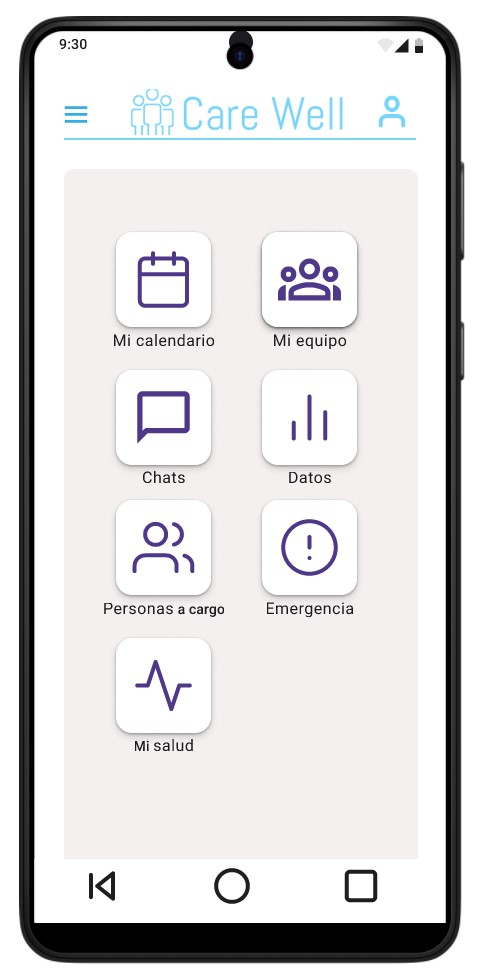
\includegraphics[width=0.25\textwidth]{Imagenes/MenuPrincipal.jpg}
    \end{wrapfigure}
    \par \textbf{CareWell} está pensada para usuarios de cualquier edad que deseen llevar un control personal de salud para sí mismos o alguien cercano, así como también orientada a usuarios que tengan a cargo o se dediquen al cuidado de personas dependientes que requieren especial atención y seguimiento.
    \par En función de los usuarios a los que apuntamos, la app debe cumplir con los siguientes puntos.
    \subsection{Interfaz sencilla e intuitiva}
    \par Fuentes grandes y de fácil legibilidad son prioridad en el desarrollo de la aplicación para facilitar el acceso a personas de avanzada edad.
    \par La navegación simplificada facilita al usuario el recorrido sobre las diferentes funcionalidades de la app, sin entrar en dudas o cuestionamientos de cómo utilizar la misma.
    \subsection{Accesibilidad}
    \par Los iconos grandes facilitan la identificación de las funcionalidades y minimizan el error de pulsación al intentar acceder a los diferentes menús.
    \par La aplicación ofrece además \textbf{tema claro y tema oscuro}. La elección no se realiza dentro de la aplicación: esta \textbf{adopta automáticamente la apariencia configurada en el sistema operativo} del dispositivo y acompaña sus cambios. Se optó deliberadamente por no incorporar un selector propio, para evitar que el usuario deba configurar dos veces la misma preferencia y para que la aplicación resulte coherente con el resto de las que utiliza.
    \par Esta decisión responde a un criterio de accesibilidad antes que estético. El tema oscuro reduce la fatiga visual y resulta especialmente pertinente en el contexto de uso de la aplicación, donde es frecuente que el cuidador deba consultarla o registrar información \textbf{durante la noche} —por ejemplo, ante una toma de medicación nocturna o un episodio de salud—, momentos en los que una pantalla clara resulta molesta tanto para quien la utiliza como para la persona bajo cuidado que descansa. Del mismo modo, beneficia a los usuarios con sensibilidad a la luz. En ambos temas se preservan los niveles de contraste necesarios para sostener la legibilidad que persigue el diseño general.
    \subsection{Seguridad y privacidad}
    \par Dado que la aplicación gestiona datos personales y de salud, el acceso se apoya en \textbf{credenciales propias} del usuario (correo electrónico y contraseña), sin depender de proveedores de identidad externos. El alta de una cuenta exige la \textbf{verificación del correo electrónico} mediante un código de un solo uso de seis dígitos, con vigencia acotada y límites de intentos y de reenvíos, de modo que solo pueda activarse una cuenta quien efectivamente controle la casilla declarada (véase la sección \textit{Verificación de correo electrónico}).
    \par Una vez autenticado, el usuario obtiene un \textbf{token de sesión} que acompaña cada operación contra el servidor, y el acceso a la información se resuelve mediante un \textbf{control de acceso basado en roles y permisos} (RBAC): lo que cada responsable o cuidador puede ver y hacer sobre una persona a cargo depende de su rol y del conjunto de permisos que le fueron otorgados (véase la sección \textit{Catálogo de permisos del sistema}). El propio usuario conserva siempre acceso completo sobre sus propios datos.
    \par En materia de privacidad, la aplicación aplica el criterio de \textbf{minimización de datos}: se recolecta y se transmite únicamente la información necesaria para prestar el servicio, las comunicaciones viajan sobre canales cifrados y las bajas de asignaciones de cuidado se realizan de forma lógica, preservando la trazabilidad sin exponer información a quien ya no forma parte del equipo. El usuario puede, además, \textbf{eliminar su cuenta} desde la propia aplicación (véase la sección \textit{Configuración}). El tratamiento de los datos se rige por lo expuesto en las secciones \textit{Términos y condiciones de la aplicación} y \textit{Política de privacidad}.
    \par El \textbf{acceso mediante plataformas de terceros} —por ejemplo, inicio de sesión con Google o vinculación de cuentas de Gmail— constituye una \textbf{integración reservada a futuro} y no forma parte del alcance de esta versión.
    \subsection{Lectura asistida de la información}
    \par Una de las dificultades relevadas es que, aun teniendo la información centralizada, al cuidador le resulta costoso \textbf{interpretarla}: los registros de salud, hábitos y estado de ánimo se acumulan día a día y los cambios relevantes pueden pasar desapercibidos en el uso cotidiano. Por ello, el diseño no se limita a mostrar los datos, sino que incorpora dos mecanismos que los \textbf{elaboran} para el usuario.
    \par El primero son las \textbf{Observaciones de bienestar}, que analizan de forma automática los registros históricos de la propia persona y advierten sobre patrones recientes —un ánimo bajo sostenido, una tendencia al deterioro, el abandono de un hábito o una caída en su cumplimiento— comparando siempre a la persona contra su propio historial. Se presentan como observaciones redactadas en lenguaje llano, sin afirmar causas ni conclusiones clínicas (véase la sección \textit{Observaciones de bienestar}).
    \par El segundo es el \textbf{Resumen diario}, accesible desde el menú principal, que consolida en un texto narrativo los eventos de salud, los hábitos de vida y los estados de ánimo registrados para la persona de contexto, de modo que el cuidador comprenda de un vistazo la situación de cuidado sin recorrer módulo por módulo (véase la sección \textit{Resumen diario de la persona a cargo}).
    \par Ambos mecanismos ayudan al cuidador a observar patrones, aportan información de respaldo para las consultas con profesionales de la salud y facilitan la toma de decisiones informadas respecto de la atención y el cuidado diario. La visualización de esta información mediante \textbf{gráficos y reportes estadísticos} constituye una mejora reservada para iteraciones posteriores.
    \subsection{Prototipo}
    \par Link de acceso al prototipo: 
    \\
    \url{https://www.figma.com/proto/astJTII0caYQpHNw2D0fNu/Care-Well?node-id=224-894&node-type=frame&t=PZPE0Pp9Ef0Die3J-1&scaling=scale-down&content-scaling=fixed&page-id=0%3A1&starting-point-node-id=109%3A332}.

    
    


    \newpage

    \printbibliography[heading=bibintoc]

\end{document}